\documentclass[a4paper,12pt, oneside]{book}

%\usepackage{fullpage}
\usepackage[italian]{babel}
\usepackage[utf8]{inputenc}
\usepackage{amssymb}
\usepackage{amsthm}
\usepackage{graphics}
\usepackage{amsfonts}
\usepackage{amsmath}
\usepackage{amstext}
\usepackage{engrec}
\usepackage{rotating}
\usepackage[safe,extra]{tipa}
\usepackage{showkeys}
\usepackage{multirow}
\usepackage{hyperref}
\usepackage{microtype}
\usepackage{enumerate}
\usepackage{braket}
\usepackage{marginnote}
\usepackage{pgfplots}
\usepackage{cancel}
\usepackage{polynom}
\usepackage{booktabs}
\usepackage{enumitem}
\usepackage{framed}
\usepackage{pdfpages}
\usepackage{pgfplots}
\usepackage{fancyhdr}
\pagestyle{fancy}
\fancyhead[LE,RO]{\slshape \rightmark}
\fancyhead[LO,RE]{\slshape \leftmark}
\fancyfoot[C]{\thepage}



\title{Analisi Matematica}
\author{UniShare\\\\Davide Cozzi\\\href{https://t.me/dlcgold}{@dlcgold}\\\\Gabriele De Rosa\\\href{https://t.me/derogab}{@derogab} \\\\Federica Di Lauro\\\href{https://t.me/f_dila}{@f\textunderscore dila}}
\date{}

\pgfplotsset{compat=1.13}
\begin{document}
\maketitle

\definecolor{shadecolor}{gray}{0.80}

\newtheorem{teorema}{Teorema}
\newtheorem{definizione}{Definizione}
\newtheorem{esempio}{Esempio}
\newtheorem{corollario}{Corollario}
\newtheorem{lemma}{Lemma}
\newtheorem{osservazione}{Osservazione}
\newtheorem{nota}{Nota}
\tableofcontents
\renewcommand{\chaptermark}[1]{%
\markboth{\chaptername
\ \thechapter.\ #1}{}}
\renewcommand{\sectionmark}[1]{\markright{\thesection.\ #1}}
\chapter{Introduzione}
\textbf{Questi appunti sono presi a lezione con la docente Rita Pini. Per quanto sia stata fatta una revisione è altamente probabile (praticamente certo) che possano contenere errori, sia di stampa che di vero e proprio contenuto.\\Per eventuali proposte di correzione effettuare una pull request. Link:} \url{https://github.com/dlcgold/Appunti}.\\
\textbf{Grazie mille e buono studio!}

\chapter{Numeri Reali}
\section{Insiemi $\mathbb{N}$, $\mathbb{Z}$, $\mathbb{Q}$}
\subsection{Numeri Naturali}
\begin{equation}
	\mathbb{N}=\{1,2,3,...\}
\end{equation}
\subsubsection{Proprietà su $\mathbb{N}$}
\begin{itemize}
\item somma $\longleftrightarrow n,m \in \mathbb{N} \rightarrow  n+m \in \mathbb{N}$
\end{itemize}
\subsection{Numeri Interi}
\begin{equation}
	\mathbb{Z}=\{...,-3,-2,-1,0,1,2,3,...\}=\{0,\pm 1,\pm 2,\pm 3,...\}
\end{equation}
\subsubsection{Proprietà su $\mathbb{Z}$}
\begin{itemize}
\item elemento neutro=0 $\longleftrightarrow n+0 \in \mathbb{Z}, n\in \mathbb{Z}$
\item $x+n=m \in \mathbb{Z}$
\item $x \cdot n=m\mbox{ con }n,m\in\mathbb{Z}$ non ha soluzione (per esempio $\nexists x\in \mathbb{Z}: 2\cdot x=1$)
\end{itemize}
\newpage
\subsection{Numeri Razionali}
Esprimibili nella forma
\begin{equation}
	\mathbb{Q} = \{\frac{p}{q} : p\in\mathbb{Z}, q\in\mathbb{N}, q \neq 0 \}
\end{equation}
\subsubsection{Frazioni equivalenti}
Ad ogni frazione di questo tipo può essere associato un unico numero razionale.\\
Ad ogni numero razionale si associano infinite frazioni.\\
Esistono le classi di \textit{frazioni equivalenti} che esprimono tutte un solo numero razionale.\\ \textit{Criterio di uguaglianza dei fattori}:$$\frac{p}{q}=\frac{p^{'}}{q^{'}} \longleftrightarrow p \cdot q^{'}=p^{'} \cdot q$$.
\subsubsection{Proprietà su $\mathbb{Q}$}
Tra i numeri razionali sono definite le due operazioni di somma e prodotto:\\
$\forall a,b,c\in\mathbb{Q}$:
\begin{itemize}
	\item Proprietà commutativa
		\begin{itemize}
			\item $a+b=b+a$
			\item $a \cdot b=b \cdot a$
		\end{itemize}
	\item Proprietà associativa
		\begin{itemize}
			\item $(a+b)+c=a+(b+c)$
			\item $(a\cdot b)\cdot c=a\cdot(b\cdot c)$
		\end{itemize}
	\item Elemento neutro
		\begin{itemize}
			\item $a+0=0+a=a$
			\item $a\cdot 1=1\cdot a=a$
		\end{itemize}
	\item Opposto / Inverso (o reciproco)
		\begin{itemize}
			\item $a+(-a)=0$
			\item $a\cdot\frac1{a}=1$, se $a\neq0$
		\end{itemize}
	\item Proprietà distributiva
		\begin{itemize}
			\item $(a+b)\cdot c=ac+bc$
		\end{itemize}
\end{itemize}
\subsection{Rappresentazione di $\mathbb{Q}$ come allineamento decimale}
Essendo $\mathbb{Q}$ rappresentabile come:
$$\mathbb{Q} = \{\frac{p}{q} : p\in\mathbb{Z}, q\in\mathbb{N}, q \neq 0 \}$$ si può associare ad ognu numero razionale infinite frazioni. Da qui si può costruire la \textit{rappresentazione con allineamenti decimali} di un numero razionale. per esempio:
$$\frac{11}{6}=1+\frac{5}{6} \mbox{ e } \frac{5}{6}=\frac{50}{60}=\frac{8\cdot 6+2}{60}=\frac{8}{10}+\frac{2}{60}$$
quindi: $$\frac{11}{6}=1+\frac{8}{10}+\frac{2}{60}$$
Si procede scomponendo le frazioni in modo da avere a denominatori le potenze di $10$ a partire da $1$. Quindi ad ogni razionale corrisponde un \textbf{unico} alineamento decimale (\textbf{finito} se il resto è da un certo punto in poi nullo, \textbf{periodico} se la parte decimale si ripete dopo un po' infinite volte). I resti delle divisioni sono quindi sempre limitati, compredi tra $0$ e $q-1$ ($q$ è il quoziente), se il resto è, dopo un po', nullo si ha un allineamento finito, se si ripete dopo un po' l'allineamento è periodico.\\Tra gli allineamenti decimali e i numeri razionali si ha una \textit{corrispondenza biunivoca}.
\subsubsection{Campo}
Le operazioni di somma e prodotto sono chiuse rispetto a  $\mathbb{Z}$, ovvero data una coppia di numeri razionali restituiscono come risultato un numero razionale.\\
L'insieme $(\mathbb{Q},+,\cdot)$ è un \textit{campo}, in quanto $(\mathbb{Q},+)$ è un \textit{gruppo Abeliano} (ovvero la somma è commutitativa e associativa e inoltre esiste l'elemento neutro, $0$) e anche $(\mathbb{Q},\cdot)$ è un \textit{gruppo abeliano} (ovviamente con elemento neutro $1$) e si ha che la moltiplicazione è distributiva rispetto all'addizione.
Il campo $\mathbb{Q}$ è inoltre un \textit{insieme ordinato} (\textbf{campo ordinato}): è definita infatti una \textit{relazione d'ordine}: per ogni coppia di numeri $(a,b)\in\mathbb{Q}\times\mathbb{Q}$ si può verificare infatti una e una sola tra le condizioni
$$a<b,\qquad a>b,\qquad a=b,$$
con le seguenti proprietà che collegano all'ordinamento le operazioni di campo:
\begin{itemize}
	\item Se $a<b$
	\begin{itemize}
		\item $\forall c, a+c<b+c$
		\item $\forall c>0, a\cdot c<b\cdot c$
		\item $\forall c<0, a\cdot c>b\cdot c$
	\end{itemize}
\end{itemize}
Nota: $\mathbb{N}$ e $\mathbb{Z}$ non sono campi; su $\mathbb{N}$ non è possibile definire opposto e reciproco, mentre su $\mathbb{Z}$ non è possibile definire il reciproco.

\section{Insieme $\mathbb{R}$}
L'insieme dei numeri razionali si può rappresentare su una retta euclidea orientata, però non basta per descrivere tutte le lunghezze.\\
Ad esempio il numero $\sqrt{2}$, che corrisponde alla misura della diagonale di un quadrato di lato 1, non è razionale.
\begin{teorema}
Non esiste alcun numero $r\in\mathbb{Q}$ tale che $r^2=2$.
\end{teorema}
\begin{proof}
Si supponga che esista un numero $r=p/q$ il cui quadrato è 2.\\
I numeri $p,q\in\mathbb{N}$ poiché $r$ è positivo, e sono primi tra loro.\\
Allora risulta
$$\Big(\frac{p}{q}\Big)^2=2,$$
cioè $p^2=2q^2$.\\
Essendo $2q^2$ pari (multiplo di $2$), anche $p^2$ lo deve essere. Di conseguenza anche $p$.\\
Quindi esiste un numero $m\in\mathbb{N}$ tale che $p=2m$, da cui segue che $4m^2=2q^2$; semplificando $2m^2=q^2$.\\
Ne deriva che anche $q^2$ è pari (multiplo di $2$). E di conseguenza $q$.\\
Questo è assurdo perché contrasta con l'ipotesi che $p$ e $q$ non abbiano fattori comuni.
\end{proof}
\begin{teorema}
Non esiste alcun numero $r\in\mathbb{Q}$ tale che $r^2=5$.
\end{teorema}
\begin{proof}
Si procede per assurdo ipotizzando che $\exists r\in \mathbb{Q}:r^2=5$.
si definisce $r=\left(\frac{p}{q}\right)$ con $p$ e $q$ primi tra loro e $p,q\in \mathbb{N}$ in quanto $r>0$, si ha quindi:
$${\left(\frac{p}{q}\right)}^2=5\Rightarrow p^2=5\cdot q^2$$
Quindi $p^2$ è multiplo di $5$ e quindi anche $p$ lo è. Quindi:
$$\exists m\in\mathbb{N}:p=5\cdot m\Rightarrow\mbox{sostituisco}\Rightarrow 25\cdot m^2=5\cdot q^2\Rightarrow 5\cdot m^2=q^2$$
Ma quindi anche $q^2$, e quindi $q$, è multiplo di $5$, fattore che va contro la tesi in quanto $p$ e $q$ sono primi tra loro.
\end{proof}
I numeri rappresentabili solamente con allineamenti decimali infiniti e non periodici fanno parte dei \emph{numeri irrazionali} $\mathbb{I}$.\\
L'unione dei numeri razionali e degli irrazionali forma l'insieme dei numeri reali.
\begin{equation}
\mathbb{R} = \mathbb{Q} + \mathbb{I}
\end{equation}
Noto che
\begin{equation}
	\mathbb{I} = \overline{\mathbb{Q}}
\end{equation}
rispetto a $\mathbb{R}$.\\\\
$\mathbb{R}$ riempie completamente la retta euclidea.
\begin{shaded}
\begin{nota}
$\mathbb{N}_0$ è l'insieme dei naturali $\mathbb{N}$ compreso lo 0. 
\end{nota}
\end{shaded}
Tutti i numeri reali possono essere scritti come allineamenti decimali, sia finiti che infiniti, periodici o non periodici, nella forma
$$\pm c_0,\,c_1c_2c_3\dots$$
dove $c_0\in\mathbb{N}_0$ e $c_1,c_2,\dots$ sono cifre in una serie infinita o finita.
\begin{shaded}
\begin{nota}
Un allinamento di periodo 9 non esiste. Per definizione è il valore subito superiore.
\end{nota}
\end{shaded}
Anche per i numeri reali valgono le operazioni di somma e prodotto come definite in $\mathbb{Q}$, e le proprietà di ordinamento, quindi anche $(\mathbb{R},+,\cdot)$ è un \textbf{campo ordinato}.
\section{Limiti di un insieme ordinato}
\subsection{Maggiorante}
\begin{definizione}
Sia $A \subseteq \mathbb{Q}, A \neq \emptyset$.\\
Si dice che A è \textbf{superiormente limitato} se $\exists\alpha\in\mathbb{R}\colon x\leq\alpha$ $\forall x\in A$.\\
$\alpha$ è \emph{maggiorante} di $A$.
\end{definizione}
\subsection{Minorante}
\begin{definizione}
Sia $A \subseteq \mathbb{Q}, A \neq \emptyset$.\\
Si dice che A è \textbf{inferiormente limitato} se $\exists\beta\in\mathbb{R}\colon x\geq\beta$ $\forall x\in A$.\\
$\beta$ è \emph{minorante} di $A$.
\end{definizione}
\subsection{Massimo}
\begin{definizione}
Si dice che $A$ ha \textit{massimo} se $\exists \overline{x} \in A \colon x \leq \overline{x}, \forall x \in A$.
\end{definizione}
\begin{nota}
Il massimo, se esiste, appartiene all'insieme: $max \in A$
\end{nota}
\begin{osservazione}
Il massimo, se esiste, è unico e corrisponde al minore di tutti i maggioranti di $A$.
\end{osservazione}
\subsection{Minimo}
\begin{definizione}
Si dice che $A$ ha \textit{minimo} se $\exists x^{'} \in A \colon x^{'} \leq x, \forall x \in A$.
\end{definizione}
\begin{nota}
Il minimo, se esiste, appartiene all'insieme: $min \in A$
\end{nota}
\begin{osservazione}
Il minimo, se esiste, è unico e corrisponde al maggiore di tutti i minoranti di $A$.
\end{osservazione}
\subsection{Estremo superiore}
\begin{definizione}
Sia $A\subseteq\mathbb{R}$, $A \neq \emptyset$, $A$ superiormente limitato.\\
Si chiama \emph{estremo superiore} di $A$ il numero $\alpha\in\mathbb{R}$ minimo dei maggioranti di $A$.
\end{definizione}
\begin{equation}
	\alpha=\sup A
\end{equation}
\begin{nota}
L'estremo superiore può talvolta anche coincidere con il massimo.\\
Ad esempio negli intervalli chiusi.\\
Se un insieme ha un massimo, tale valore è anche l'estremo superiore. Il viceversa invece non vale: se un insieme ha l'estremo superiore non necessariamente ha anche un massimo;\\
Se esistono entrambi, ovviamente non possono che coincidere.
\end{nota}
\begin{osservazione}
Un estremo superiore ($\alpha$), deve soddisfare queste condizioni:
\begin{itemize}
\item deve essere un maggiorante: $x\leq\alpha$ $\forall x\in A$
\item deve essere il minore dei maggioranti: $\forall\epsilon>0$, $\exists\tilde{a}\in A\colon\alpha-\epsilon<\tilde{a}\leq\alpha$\\
Spostandosi a sinistra di $\alpha$ (nell'insieme $A$) di una quantità arbitrariamente piccola $\epsilon$ si devono trovare solamente elementi di $A$, e non altri maggioranti.
\end{itemize}	
\end{osservazione}
\subsection{Estremo inferiore}
\begin{definizione}
Sia $A\subseteq\mathbb{R}$, $A \neq \emptyset$, $A$ inferiormente limitato.\\
Si chiama \emph{estremo inferiore} di $A$ il numero $\beta\in\mathbb{R}$ massimo dei minoranti di $A$.
\end{definizione}
\begin{equation}
	\beta=\inf A
\end{equation}
\begin{nota}
L'estremo inferiore può talvolta anche coincidere con il minimo.\\
Ad esempio negli intervalli chiusi.\\
Se un insieme ha un minimo, tale valore è anche l'estremo inferiore. Il viceversa invece non vale: se un insieme ha l'estremo inferiore non necessariamente ha anche un minimo;\\
Se esistono entrambi, ovviamente non possono che coincidere.
\end{nota}
\begin{osservazione}
Un estremo inferiore ($\beta$), deve soddisfare queste condizioni:
\begin{itemize}
\item deve essere un minorante: $\beta\leq x$ $\forall x\in A$
\item deve essere il maggiore dei minoranti: $\forall\epsilon>0$, $\exists\tilde{a}\in A\colon\alpha\geq\tilde{a}>\alpha+\epsilon$\\
Spostandosi a destra di $\alpha$ (nell'insieme $A$) di una quantità arbitrariamente piccola $\epsilon$ si devono trovare solamente elementi di $A$, e non altri minoranti.
\end{itemize}	
\end{osservazione}
\subsection{Proprietà dell'estremo superiore}
\begin{teorema}[Proprietà dell'estremo superiore]
Ogni sottoinsieme di $\mathbb{R}$ limitato superiormente possiede sempre un estremo superiore.
\end{teorema}
\begin{nota}
$\mathbb{Q}$, al contrario di $\mathbb{R}$ non possiede tale proprietà.\\
Esiste almeno un sottoinsieme di $\mathbb{Q}$ che, pur essendo superiormente limitato, non ammette un estremo superiore.
\end{nota}
A partire da questa proprietà si può definire l'operazione di addizione tra due allineamenti infiniti di numeri reali.
Per farlo, si costruiscono le somme dei troncati di due numeri approssimati ogni volta ad una cifra decimale in più: queste somme dei troncati saranno sempre minori della somma reale dei due numeri, e formano una famiglia di elementi che ha un elemento superiore; tale estremo è la somma dei due numeri cercata.
\subsection{Densità di $\mathbb{R}$}
\begin{teorema}[Densità di $\mathbb{R}$]
Assegnati due qualunque numeri reali distinti, si possono sempre trovare tra di essi un numero razionale e un numero irrazionale.
\begin{equation}
\forall a,b\in \mathbb{R}\mbox{ } a<b,	
\begin{matrix}
	\exists r\in \mathbb{Q} \mbox{ tale che } a<r<b \\ 
	\exists r^{'}\in \mathbb{I} \mbox{ tale che } a<r^{'}<b
\end{matrix}
\end{equation}
\end{teorema}
Il procedimento si può iterare infinite volte. Ne segue che tra ogni coppia di numeri reali esistono infiniti numeri razionali e infiniti numeri irrazionali.\\
Allora gli insiemi $\mathbb{Q}$ e $\mathbb{I} (= \mathbb{R}\setminus\mathbb{Q})$ sono densi in $\mathbb{R}$.
\newpage
\subsection{Parte intera e valore assoluto}
\subsubsection{Parte intera}
La funzione \textit{Parte intera} associa d ogni $x\in\mathbb{R}$ il più grande intero $z\in\mathbb{Z}$ con $z\leq x$. Si ha la seguente notazione per la parte intera di $x$:
$$\lfloor x \rfloor$$
\begin{center}
\begin{tikzpicture}
\begin{axis}[width= 8cm,height= 8cm,xmin=-3, xmax=3,ymin=-2, ymax=2,axis lines= middle,xtick={-3,-2,-1,0,1,2,3}, ytick={-3,-2,-1,0,1,2,3},title=Funzione Parte Intera]
\addplot+[mark=none,blue] coordinates {(2,2)(3,2)};
\addplot+[mark=*,black] coordinates {(3,2)};
\addplot+[mark=none,blue] coordinates {(1,1)(2,1)};
\addplot+[mark=*,black] coordinates {(2,1)};
\addplot+[mark=none,blue] coordinates {(-1,-1)(0,-1)};
\addplot+[mark=*,black] coordinates {(0,-1)};
\addplot+[mark=none,blue] coordinates {(0,0)(1,0)};
\addplot+[mark=*,black] coordinates {(1,0)};
\addplot+[mark=none,blue] coordinates {(-3,-3)(-2,-3)};
\addplot+[mark=*,black] coordinates {(-2,-3)};
\addplot+[mark=none,blue] coordinates {(-2,-2)(-1,-2)};
\addplot+[mark=*,black] coordinates {(-1,-2)};
\end{axis}
\end{tikzpicture}
\end{center}
\subsubsection{Valore assoluto}
Il valore assoluto è una funzione che associa $x\in\mathbb{R}$ un $\alpha\in\mathbb{R}$ non negativo:
\begin{center}
 $|x|=\left\{
                \begin{array}{ll}
               	  x &\mbox{ se } x\geq0\\
               	 -x &\mbox{ se } x<0
				\end{array}
				\right.$
\end{center}
$|x|$ è quindi sempre positivo.
\subsection{Proprietà archimedea}
\begin{teorema}[Proprietà archimedea]
Siano
\begin{itemize}
	\item $\alpha,\beta>0$
	\item $\alpha<\beta$
	\item $\alpha,\beta \in \mathbb{R}$
\end{itemize}
allora $\exists n \in \mathbb{N}$ tale che $n\alpha>\beta$.\\
Ovvero dopo un numero finito di "saltelli" $n\alpha$ avrà superato $\beta$.
\end{teorema}
\newpage
\section{Intervalli}
\subsection{Intervalli limitati}
\subsubsection{Intervallo chiuso}
\begin{equation}
[a,b]=\{x\in\mathbb{R}\colon a\leq x\leq b\}	
\end{equation}
\subsubsection{Intervallo aperto}
\begin{equation}
(a,b)=\{x\in\mathbb{R}\colon a<x<b\}	
\end{equation}
\subsection{Intervalli illimitati, superiormente e/o inferiormente}
\subsubsection{Intervallo chiuso}
\begin{equation}
[a,+\infty)=\{x\in\mathbb{R}\colon x>a\}
\end{equation}
\subsubsection{Intervallo aperto}
\begin{equation}
(-\infty,b)=\{x\in\mathbb{R}\colon x\leq b\}
\end{equation}
\begin{shaded}
\begin{nota}
I simboli di $-\infty$ e $+\infty$ sono solo convenzioni e non rappresentano dei numeri né appartengono all'insieme $\mathbb{R}$, ma sono compresi nell'insieme dei numeri reali \emph{esteso}:
\begin{equation}
\overline{\mathbb{R}}=\mathbb{R}\cup\{-\infty\}\cup\{+\infty\}
\end{equation}
\end{nota}
\end{shaded}
\subsection{Intervalli di $\mathbb{R}$}
Si definisce la seguente simbologia per gli intervalli in $\mathbb{R}$
\begin{itemize}
\item $(\alpha,\beta) \longleftrightarrow \{x \in \mathbb{R}: \alpha < x < \beta\}$
\item $[\alpha,\beta] \longleftrightarrow \{x \in \mathbb{R}: \alpha \leq x \leq \beta\}$
\item $(\alpha,\beta] \longleftrightarrow \{x \in \mathbb{R}: \alpha < x \leq \beta\}$
\item $[\alpha,\beta) \longleftrightarrow \{x \in \mathbb{R}: \alpha \leq x < \beta\}$
\item $(\alpha,+\infty) \longleftrightarrow \{x \in \mathbb{R}: x>\alpha\}$
\item $[\alpha,+\infty) \longleftrightarrow \{x \in \mathbb{R}: x\geq\alpha\}$
\item $(-\infty,\alpha) \longleftrightarrow \{x \in \mathbb{R}: x<\alpha\}$
\item $(-\infty,\alpha] \longleftrightarrow \{x \in \mathbb{R}: x\leq\alpha\}$
\item $\mathbb{R}=(-\infty,+\infty)$
\end{itemize}
\subsubsection{Sottoinsiemi connessi}
Gli intervalli sono \textit{sottoinsiemi connessi}: dati due punti dell'insieme, tutti i punti contenuti nel segmento che li congiunge sono contenuti nell'insieme.
\begin{osservazione}
Qualora ci fosse un 'salto' non sarebbe un sottoinsieme connesso.
\end{osservazione}
\section{Topologia di $\mathbb{R}$}
\subsection{Intorno}
\begin{definizione}
Sia $\overline{x} \in A \subseteq \mathbb{R}$ si chiama \emph{intorno circolare} (o \emph{bolla}) di $\overline{x}$ di raggio $r > 0$ l'insieme
\begin{equation}
B(\overline{x},r)= (\overline{x} - r, \overline{x} + r)
\end{equation}
\end{definizione}
\subsection{Classificazione dei Punti}
Il punto $\overline{x}\in A \subseteq \mathbb{R}$ si dice:
\begin{itemize}
\item \textbf{interno} ad $A$ se esiste un intorno, centrato in $\overline{x}$, tutto contenuto in $A$: $$\exists r>0\colon B(\overline{x},r)\subset A;$$
\item \textbf{esterno} ad $A$ se esiste un intorno, centrato in $\overline{x}$, tutto contenuto nel complemento di A: $$\exists r>0\colon B(\overline{x},r)\subset\overline{A};$$
\item \textbf{di frontiera} se non è interno né esterno, ossia se ogni intorno centrato in $\overline{x}$ contiene sia punti di $A$ sia punti di $\overline{A}$:
$$\forall r>0:\left\{
                \begin{array}{ll}
					B(\overline{x},r)\cap A\neq\emptyset\\
					B(\overline{x},r)\cap\overline{A}\neq\emptyset
				\end{array}
				\right.$$
\end{itemize}
\begin{osservazione}
	Questa classificazione è disgiuntiva ed esaustiva, perché ogni punto rientra sempre in una soltanto delle tre categorie.	
\end{osservazione}
\begin{shaded}
L'insieme dei punti interni di $A$ si chiama \emph{interno} e si indica con ${A}^{\circ}$, che non coincide necessariamente con l'insieme stesso.\\

L'insieme dei punti di frontiera, che possono o meno appartenere all'insieme (non si può stabilire a priori) si chiama \emph{frontiera} e si indica con $\partial A$.
\end{shaded}
\subsection{Punto di accumulazione}
\begin{definizione}
Sia $A \subseteq \mathbb{R}$, $r>0$\\
$\overline{x}$ è un \emph{punto di accumulazione} di A se, per ogni intorno di $\overline{x}$, esiste almeno un altro punto $x$ ($ \neq \overline{x}$) $\in A$ interno all'intorno.
\begin{equation}
\forall B(\overline{x},r) \mbox{  } \exists \mbox{ almeno un punto x} \in A, x \neq \overline{x} \mbox{ tale che } x \in B(\overline{x},r)
\end{equation}
\end{definizione}
\subsection{Punto isolato}
\begin{definizione}
Sia $A \subseteq \mathbb{R}$, $r>0$\\
$\overline{x}$ è un \emph{punto isolato} di A se per ogni intorno di $\overline{x}$, non esiste nessun altro punto $x$ ($ \neq \overline{x}$) $\in A$ interno all'intorno; solo $\overline{x}$ appartiene all'intorno.
\begin{equation}
\exists B(\overline{x}, r) \colon \{\overline{x}\} = A \cap B(\overline{x}, r)
\end{equation}
\end{definizione}
\chapter{Funzioni}
\begin{equation}
	f: x \rightarrow y
\end{equation}
con 
\begin{itemize}
	\item $x \in X \subseteq \mathbb{R}$
	\item $y = f(x) \in Y \subseteq \mathbb{R}$
\end{itemize}
\begin{shaded}
\begin{itemize}
	\item $X \rightarrow $ dominio di $f$
	\item $Y \rightarrow $ codominio di $f$
	\item $y = f(x) \rightarrow $ immagine di x
	\item $f(x) = \{ y = f(x), x \in X \} \rightarrow $ insieme immagine di x
\end{itemize}
\end{shaded}
\section{Grafico di funzione}
Si può dire che per disegnare una funzione si ha la seguente definizione: $$gr(f)=\{(x,y)\in X\times Y: y=f(x)\}$$
\subsection{grafici fondamentiali}
\begin{center}
\begin{tikzpicture}
\begin{axis}[width= 8cm,height= 8cm,xmin=-3, xmax=3,ymin=-3, ymax=3,axis lines= middle,title=Qualche $\alpha\cdot x$]
\addplot[black,line width=1pt]{2*x};
\node[pin=30:{$2\cdot x$}]at (axis cs:1,2) {};
\addplot[black,line width=1pt]{x};
\node[pin=30:{$x$}]at (axis cs:1,1) {};
\addplot[black,line width=1pt]{-x};
\node[pin=-30:{$-x$}]at (axis cs:1,-1) {};
\addplot[black,line width=1pt]{-2*x};
\node[pin=-30:{$-2\cdot x$}]at (axis cs:1,-2.2) {};
\end{axis}
\end{tikzpicture}
\end{center}

\begin{tikzpicture}
\begin{axis}[width= 8cm,height= 8cm,xmin=-3, xmax=3,ymin=-3, ymax=3,axis lines= middle,title=Grafico di $x^2$]
\addplot[black,line width=1pt,samples=100]{x^2};
\end{axis}
\end{tikzpicture}
~
\begin{tikzpicture}
\begin{axis}[width= 8cm,height= 8cm,xmin=-3, xmax=3,ymin=-3, ymax=3,axis lines= middle,title=Grafico di $x^3$]
\addplot[black,line width=1pt, samples =100]{x^(3)};
\end{axis}
\end{tikzpicture}
\begin{center}\textit{Gli $n$ dispari permettono $f(x)$ negative}\end{center}

\begin{tikzpicture}
\begin{axis}[width= 8cm,height= 8cm,axis lines= middle,title=Qualche $x^{\frac{1}{n}}$]
\addplot[black,line width=1pt, samples=100]{x^0.5};
\node[pin=-30:{$x^{\frac{1}{2}}$}]at (axis cs:1.5,1.1) {};
\addplot[black,line width=1pt,samples=100]{-x^(1/2)};
\node[pin=-50:{$-x^{\frac{1}{2}}$}]at (axis cs:1.1,-1.1) {};
\end{axis}
\end{tikzpicture}
~
\begin{tikzpicture}
\begin{axis}[width= 8cm,height= 8cm,axis lines= middle,title=Grafico di $\frac{1}{x}$]
\addplot[black,line width=1pt, samples=100]{1/(x)};
\end{axis}
\end{tikzpicture}

\section{Caratteristiche particolari}
\subsection{Funzione iniettiva}
\begin{definizione}
Una funzione si dice \emph{iniettiva} se associa ad elementi distinti del dominio elementi distinti del codominio.
\begin{equation}
\forall x_1,x_2\in X, x_1\neq x_2 \Rightarrow f(x_1)\neq f(x_2)
\end{equation}
\end{definizione}
\subsection{Funzione suriettiva}
\begin{definizione}
Una funzione si dice \emph{suriettiva} quando ogni elemento del codominio è immagine di almeno un elemento del dominio; di conseguenza quando l’insieme delle immagini coincide con il codominio.
\begin{equation}
f(X)=Y=\mathbb{R}
\end{equation}
\end{definizione}
\subsection{Funzione biunivoca (o biettiva)}
Una funzione si dice \emph{biunivoca} (o \emph{biettiva}) quando è sia iniettiva che suriettiva.
\section{Restrizione del dominio}
\begin{definizione}
Sia $f:X\rightarrow Y$ e sia $X^{'}\subset X$.\\
Sia chiama \emph{restrizione} di $f$ a $X^{'}$, e si indica con $f|_{X^{'}}$, la funzione
\begin{equation}
f|_{X^{'}}:x^{'}\rightarrow y,\mbox{ } x^{'}\in X^{'} \rightarrow f(x^{'})
\end{equation}
\end{definizione}
\section{Simmetrie particolari}
\subsection{Funzione pari}
\begin{definizione}
Sia $f:D\subseteq \mathbb{R} \rightarrow \mathbb{R}$.\\
$f$ è \emph{pari} se 
\begin{equation}
	f(-x)=f(x), \mbox{ } \forall x \in D
\end{equation}
\end{definizione}
\begin{nota}
Una funzione \emph{pari} è simmetrica rispetto all'asse delle y.
\end{nota}
\subsection{Funzione dispari}
\begin{definizione}
Sia $f:D\subseteq \mathbb{R} \rightarrow \mathbb{R}$.\\
$f$ è \emph{dispari} se 
\begin{equation}
	f(-x)=-f(x), \mbox{ } \forall x \in D
\end{equation}
\end{definizione}
\begin{nota}
Una funzione \emph{dispari} è simmetrica rispetto all'origine.
\end{nota}
\begin{shaded}
\begin{nota}
Vale sempre la seguente uguaglianza:
$$\frac{\mbox{funzione dispari}}{\mbox{funzione pari}} = \mbox{funzione dispari}$$
\end{nota}	
\end{shaded}
\section{Funzione periodica}
\begin{definizione}
Si dice che una funzione $f$ è \emph{periodica} di periodo $P$ se $P$ è il minimo numero positivo tale che
\begin{equation}
f(x+P) = f(x)
\end{equation}
\end{definizione}
\section{Composizione di funzioni}
\begin{definizione}
Siano $f: X \rightarrow Y$ e $g: Y \rightarrow Z$ due funzioni tale che 
\begin{equation}
x \longrightarrow y = f(x) \longrightarrow g(f(x))
\end{equation}
si chiama \emph{composizione} di $f$ con $g$ la funzione
\begin{equation}
g \circ f: X\rightarrow Z
\end{equation} 
con 
\begin{equation}
(g\circ f)(x)=g(f(x))
\end{equation}
\end{definizione}
\section{Funzione inversa}
\begin{definizione}
Le funzioni biunivoche sono invertibili.\\
Si definisce così la \textbf{funzione inversa} di $f(x)$:
\begin{equation}
f^{-1}:Y\rightarrow X
\end{equation}
con 
\begin{equation}
	x = f^{-1}(y)
\end{equation}
\end{definizione}
\subsection{Proprietà delle funzioni inverse}
\subsubsection{Funzione identica}
\begin{definizione}
Se $f:X\rightarrow Y$ e $f^{-1}:Y\rightarrow X$,\\
allora $f^{-1}\circ f: X \rightarrow X$ è la \emph{funzione identica}, tale che
\begin{equation}
(f^{-1}\circ f)(x)=x
\end{equation}
\end{definizione}
\subsubsection{Commutatività della composizione di $f$ con $f^{-1}$}
\begin{equation}
f^{-1}\circ f= f\circ f^{-1}
\end{equation}
\subsubsection{Proprietà grafiche delle funzioni inverse}
Le funzioni inverse sono sempre simmetriche rispetto alla bisettrice del $\mathbf{I}$ e $\mathbf{III}$ quadrante.
\subsection{Invertibilità parziale}
Alcune funzioni sono invertibili solo in una loro restrizione.
\begin{esempio}
$\sin{x}$ e $\cos{x}$ sono invertibili solamente dopo aver ristretto il dominio in un intervallo che renda la funzione biettiva: $[-\frac{\pi}{2}, \frac{\pi}{2}]$.\\\\
$\sin{x}: (-\infty, +\infty) \rightarrow (-1, +1)$ non è invertibile.\\
$\sin{x}: [-\frac{\pi}{2}, \frac{\pi}{2}] \rightarrow (-1, +1)$ è invertibile.
\end{esempio}
\subsection{Altri grafici fondamentali}

\begin{tikzpicture}
\begin{axis}[width= 8cm,height= 8cm,axis lines= middle,title=Grafico di $2^x$]
\addplot[black,line width=1pt, samples =100]{2^(x)};
\end{axis}
\end{tikzpicture}
~
\begin{tikzpicture}
\begin{axis}[width= 8cm,height= 8cm,axis lines= middle,title=Grafico di ${-2}^x$]
\addplot[black,line width=1pt, samples =100]{-2^x};
\end{axis}
\end{tikzpicture}

\begin{tikzpicture}
\begin{axis}[width= 8cm,height= 8cm,axis lines= middle,title=Grafico di $\log x$]
\addplot[black,line width=1pt, samples =100]{ln(x)};
\end{axis}
\end{tikzpicture}
~
\begin{tikzpicture}
\begin{axis}[width= 8cm,height= 8cm,axis lines= middle,title=Grafico di $-\log x$]
\addplot[black,line width=1pt, samples =100]{-ln(x)};
\end{axis}
\end{tikzpicture}

\begin{tikzpicture}
\begin{axis}[width= 8cm,height= 8cm,axis lines= middle,title=Grafico di $e^x$]
\addplot[black,line width=1pt, samples =100]{e^(x)};
\end{axis}
\end{tikzpicture}
~
\begin{tikzpicture}
\begin{axis}[width= 8cm,height= 8cm,axis lines= middle,title=Grafico di $-e^x$]
\addplot[black,line width=1pt, samples =100]{-e^(x)};
\end{axis}
\end{tikzpicture}

\begin{tikzpicture}
\begin{axis}[width= 8cm,height= 8cm,axis lines= middle,title=Grafico di $\cos x$]
\addplot[black,line width=1pt, samples =100]{cos(deg(x))};
\end{axis}
\end{tikzpicture}
~
\begin{tikzpicture}
\begin{axis}[width= 8cm,height= 8cm,axis lines= middle,title=Grafico di $\sin x$]
\addplot[black,line width=1pt, samples =100]{sin(deg(x))};
\end{axis}
\end{tikzpicture}
\begin{center}
\begin{tikzpicture}
\begin{axis}[width=8cm,height=8cm,xmin=-4.72,xmax=4.71,ymin=-4.5,ymax=4.5,axis lines= middle,title=Grafico di $\tan x$]
\addplot[black,line width=1pt, samples =100]{tan(deg(x))};
\end{axis}
\end{tikzpicture}
\end{center}


\begin{tikzpicture}
\begin{axis}[width= 8cm,height= 8cm,axis lines= middle,title=Grafico di $\arccos x$]
\addplot[black,line width=1pt,domain=-1:1, samples =101,trig format=rad]{acos(x)};
\end{axis}
\end{tikzpicture}
~
\begin{tikzpicture}
\begin{axis}[width= 8cm,height= 8cm,axis lines= middle,title=Grafico di $\arcsin x$]
\addplot[black,line width=1pt,domain=-1:1, samples =101,trig format=rad]{asin(x)};
\end{axis}
\end{tikzpicture}

\begin{center}
\begin{tikzpicture}
\begin{axis}[width= 8cm,height= 8cm,axis lines= middle,title=Grafico di $\arctan x$]
\addplot[black,line width=1pt, samples =101,trig format=rad]{atan(x)};
\end{axis}
\end{tikzpicture}
\textit{con} $\arctan x :(-\infty,+\infty)\to(-\frac{\pi}{2},+\frac{\pi}{2})$
\end{center}
Si definiscono infine le funzioni iperboliche:
\begin{itemize}
\item $\sinh x= \frac{e^x-e^{-x}}{2}$
\item $\cosh x= \frac{e^x+e^{-x}}{2}$
\item $\tanh x= \frac{e^x-e^{-x}}{e^x+e^{-x}}$
\end{itemize} 
\chapter{Successioni}
\section{Definizione di successione}
Si chiama successione una funzione dall'insieme dei numeri naturali $\mathbb{N}$ all'insieme dei numeri reali $\mathbb{R}$.
\begin{equation}
	f\colon\mathbb{N}\to \mathbb{R}
\end{equation}
\subsection{Simbologia per le successioni}
Una successione viene indicata con $\{a_n\}_{n=1}^{\infty}$ e $\{ a_1, a_2, ..., a_n, ... \}$, o per semplicità con $\{a_n\}$. A livello grafico una successione si può rappresentare come un insieme di punti:
\begin{center}
\begin{tikzpicture}
\begin{axis}[width= 8cm,height= 8cm,axis lines= middle,title=Grafico di $1/n$]
\addplot[mark=*] coordinates {(1,1)};
\addplot[mark=*] coordinates {(2,0.5)};
\addplot[mark=*] coordinates {(3,0.3)};
\addplot[mark=*] coordinates {(4,0.25)};
\addplot[mark=*] coordinates {(5,0.2)};
\addplot[mark=*] coordinates {(6,0.16)};
\addplot[mark=*] coordinates {(7,0.14)};
\end{axis}
\end{tikzpicture}
\end{center}
\subsubsection{Termine generale} 
L'immagine $f(n)$, con $n \in \mathbb{N}$, viene indicata con $a_n$.
\begin{equation}
	f(n) = a_n
\end{equation}
$a_n$ si chiama \emph{termine generale} della successione.\\
Sebbene il termine generale indichi l'immagine della successione e non la successione stessa, per convenzione si può usare per indicare la successione.
\section{Successioni monotone}
Una successione $\{a_n\}$ può essere:
\begin{itemize}
\item crescente (o crescente in senso stretto), se $\forall n$ si ha $a_n<a_{n+1}$;
\item non decrescente (o crescente in senso lato), se $\forall n$ si ha $a_n\leq a_{n+1}$;
\item decrescente (o decrescente in senso stretto), se $\forall n$ si ha $a_n>a_{n+1}$;
\item non crescente (o decrescente in senso lato), se $\forall n$ si ha $a_n\geq a_{n+1}$.
\end{itemize}
Se una di queste proprietà è verificata, la successione è \textit{monotona}.	
\begin{shaded}
\begin{nota}
Si dice che una proprietà per una successione vale \textbf{definitivamente} se esiste un valore $\exists n_0$ tale che $\forall n > n_0$ la proprietà è verificata.
\end{nota}
È diverso affermare che una successione verifica una proprietà per infiniti $n$ o definitivamente.\\\\
Ad esempio, la successione a valori reali $a_n=(-1)^n$ soddisfa la proprietà $a_n=1$ per infiniti $n$, ma non definitivamente, infatti continua ad oscillare tra 1 e $-1$ e non si può stabilire un numero $n=n_0$ oltre il quale $a_n$ verifichi \textit{sempre} la proprietà.
\end{shaded}
Una successione è \emph{definitivamente monotona} se una delle precedenti proprietà vale solo per $\forall n > n_0$. In questo particolare caso le proprietà delle successioni monotone valgono solo per gli $n > n_0$.
\section{Successioni regolari}
\subsection{Successioni convergenti}
\subsubsection{Limite di successione}
\begin{definizione}
Si dice che la successione $\{a_n\} \rightarrow \ell \in \mathbb{R}$ (o, ha limite uguale a $\ell$) per $n  \rightarrow + \infty$ 
\begin{equation}
\lim_{n\to +\infty}a_n=\ell
\end{equation}
se $ \forall\epsilon > 0$, $\exists n_0 \in \mathbb{N}$ tale che $a_n \in B(\ell, \epsilon)$ $\forall n \geq n_0$.
\end{definizione}
La successione $a_n$ \textbf{converge} a $\ell$.
\subsection{Successioni divergenti}
\begin{shaded}
\begin{nota}
Sia $a \in \mathbb{R}$.\\
Si chiama \textbf{intorno di +$\infty$} un insieme del tipo $(a, +\infty)$.\\
Allo stesso modo, si chiama \textbf{intorno di -$\infty$} un insieme del tipo $(- \infty , a)$.
\end{nota}
\end{shaded}
\begin{definizione}
Si dice che la successione $\{a_n\} \rightarrow \pm \infty$
\begin{equation}
\lim_{n\to +\infty}a_n=+\infty
\end{equation}
se $\forall a \in \mathbb{R}, \exists n_0 \in \mathbb{N}$ tale che $a_n \in (a, +\infty)$ $\forall n \geq n_0$.
\end{definizione}
\section{Successioni irregolari}
Le successioni \textbf{regolari} sono quelle per cui $\exists$ un limite finito (\textit{convergenti}) e quelle il cui limite è infinito $\pm \infty$ (\textit{divergenti}).\\
Tutte le altre si dicono \textbf{irregolari}.
\section{Teorema di unicità del limite}
\begin{teorema}[di unicità del limite]
Sia $a_n$ una successione regolare.\\
Se $$\lim_{n\to +\infty}a_n=L$$ tale limite è \textbf{unico}.
\end{teorema}
Nota: per definizione di successione regolare, $L \in \mathbb{R}$ o $L = \pm \infty$.
\begin{proof}
\textbf{Per assurdo} $\exists L_1, L_2$ con $L_1 \neq L_2$\\
tali che $a_n \rightarrow L_1$ e $a_n \rightarrow L_2$.\\
\\
Supponiamo che siano $L_1, L_2 \in \mathbb{R}$ e $L_1 \leq L_2$.\\
\\ 
Sia $0 < \epsilon \leq \frac{L_2-L_1}{2} $ (ovvero $B_2(L_2, \epsilon) \wedge B_1(L_1, \epsilon) = 0$, "gli intorni non si intersecano")\\\\
$\Rightarrow \begin{matrix}
\exists n_0 \in \mathbb{N}$ tale che $L_1 - \epsilon < a_n < L_1 + \epsilon$, $\forall n \geq n_0\\ 
\exists n_1 \in \mathbb{N}$ tale che $L_2 - \epsilon < a_n < L_2 + \epsilon$, $\forall n \geq n_1
\end{matrix}$\\\\
Sia $N = max\{n_0, n_1\} \Rightarrow $ impossibile! perchè se $n \rightarrow \pm\infty $, $N$ sarebbe contemporaneamente in $B_1$ e $B_2$ e non può esserlo dato che i due intorni non si intersecano.
\end{proof}
% da dimostrare anche per L_1 finito ed L_2 infinito
\section{Successione limitata}
\begin{definizione}
Si dice che la successione $\{ a_n \}$ è limitata se l'insieme $\{ a_1, a_2, ..., a_n \}$ è un sottoinsieme limitato di $\mathbb{R}$.
\end{definizione}
\subsection{Successione convergente è limitata}
\begin{osservazione}
Sia $\{a_n\}$ una successione.\\ 
Se $\{a_n\} \rightarrow L \in \mathbb{R}$ (\textit{convergente}) $\Rightarrow \{a_n\}$ è limitata.\\
Se $\{a_n\} \rightarrow \pm \infty $ (\textit{divergente}) $\Rightarrow \{a_n\}$ non è limitata.
\end{osservazione}
% bonus
\begin{proof}[Dimostrazione bonus]
Si scelga $\epsilon=1$ come raggio dell'intorno. Sia $\ell$ il limite della successione: per ipotesi, esiste un numero intero $N$ tale che $\forall n\geq N$ risulta $a_n\in B(\ell,1)$. Allora l'insieme formato dai valori di $\{a_n\}$ per $n\geq N$ ha un diametro inferiore o uguale a 2, quindi è limitata. Allora poiché l'insieme dei valori della successione per $n<N$ è di cardinalità finita, è limitato anch'esso, quindi tutta la successione è limitata in quanto somma di due insiemi limitati.
\end{proof}
% end bonus
\begin{nota}
Il viceversa non vale. Una successione è limitata quando il suo codominio è limitato; non implica necessariamente che la successione converga ad un limite.\\
Ad esempio, la successione $a_n=(-1)^n$ limitata, ma non converge.	
\end{nota}
\section{Teorema di permanenza del segno}
\begin{teorema}[di permanenza del segno]
Sia $\{a_n\} \rightarrow L$, con $L > 0$ (eventualmente $L = +\infty$)\\
allora $a_n > 0$ definitivamente;\\
ovvero $\exists n_0$ a partire dal quale la successione è strettamente positiva.
\end{teorema}
\begin{proof}
Sia $L \in \mathbb{R}$, $L>0$. Scelgo $\epsilon=\frac{L}{2}$\\\\
Considero l'intorno di L: $(\frac{L}{2},\frac{3}{2}L)$\\\\
$\Rightarrow \exists n_0\in \mathbb{N}$ tale che $\forall n \geq n_0$, $a_n\in (\frac{L}{2},\frac{3}{2}L)=B(L,\frac{L}{2})$\\\\
in particolare $a_n>\frac{L}{2}(>0)$.
\end{proof}
% da dimostrare anche per negativi, + infinito e - infinito.


\section{Teorema del confronto (per successioni)}
\begin{teorema}[del confronto] \
\begin{enumerate}
\item Siano $\{a_n\}$, $\{b_n\}$ e $\{c_n\}$ tre successioni a valori reali, con $a_n\leq b_n\leq c_n$ definitivamente. Se le successioni $a_n$ e $c_n$ convergono entrambe ad un limite $\alpha$, allora $b_n$ ammette il limite, e tale limite coincide con $\alpha$.
\item Siano $\{a_n\}$ e $\{b_n\}$ due successioni a valori reali, con $a_n\leq b_n$ definitivamente:
	\begin{itemize}
		\item se $a_n$ diverge a $+\infty$, allora anche $b_n$ ammette il limite, che è $+\infty$;
		\item se $b_n$ diverge a $-\infty$, allora anche $a_n$ ammette il limite, che è $-\infty$.
	\end{itemize}
\end{enumerate}
\end{teorema}
\begin{proof}\
\begin{enumerate}
\item Per la convergenza di $a_n$ e $c_n$ si ha che
	\begin{itemize}
		\item $\forall\epsilon>0\;\exists n_0\colon\forall n\geq n_0\to\alpha-\epsilon<a_n<\alpha+\epsilon$;
		\item $\forall\epsilon>0\;\exists n_1\colon\forall n\geq n_1\to\alpha-\epsilon<c_n<\alpha+\epsilon$.
	\end{itemize}
Per tutti gli $n\geq\max\{n_0,n_1\}$ devono sussistere entrambe le proprietà. Allora, poiché per ipotesi $b_n$ è compreso tra le altre due successioni, risulta
\[
\alpha-\epsilon<a_n\leq b_n\leq c_n<\alpha+\epsilon,
\]
A questa relazione segue che $\alpha-\epsilon<b_n<\alpha+\epsilon$, quindi anche $b_n$ converge ad $\alpha$.
\item Nel caso in cui $a_n\to +\infty$, segue che definitivamente $a_n>M$ (con $M$ arbitrariamente grande).\\
Per ipotesi, $b_n\geq a_n$. Quindi definitivamente si ha $b_n\geq a_n>M$.\\
Ne deriva $b_n>M$, ovvero $b_n$ diverge a $+\infty$.\\\\
Analogamente si dimostra il caso in cui $b_n\to -\infty$.\qedhere
\end{enumerate}
\end{proof}
È possibile utilizzare il criterio del confronto per dimostrare l'esistenza di alcuni limiti e determinarne la convergenza o divergenza.\\
Dal teorema del confronto segue che
\begin{osservazione}
Sia $\{a_n\}$ il prodotto di due successioni $b_n$ e $c_n$. Se $b_n\to 0$ e $c_n$ è limitata, la successione $a_n=b_n\cdot c_n$ converge a 0.
\end{osservazione}
% specificare meglio cos'è
\begin{definizione}[Limiti destro e sinistro]
Sia $\{a_n\}$ una successione convergente a valori reali. Si dice che $a_n$ tende a $\ell\in\mathbb{R}$ per \emph{eccesso} (e si indica $a_n\to\ell^+$) se la successione è definitivamente compresa nell'intorno destro di $\ell$, cioè in $[\ell,\ell+\epsilon)$.
Analogamente, $a_n$ tende a $\ell\in\mathbb{R}$ per \emph{difetto} (e si indica $a_n\to\ell^-$) se la successione è definitivamente compresa nell'intorno sinistro di $\ell$, cioè in $(\ell-\epsilon,\ell]$.
\end{definizione}
\section{Teorema di esistenza del limite per s. monotone}
\begin{teorema}(Teorema di esistenza del limite per successioni monotone)\\
Tutte le successioni monotone sono regolari. Sia inoltre $\{a_n\}$ una successione a valori reali: se è monotona crescente, allora
$$\lim_{n\to +\infty} a_n=\sup\{a_n\},$$
e tale limite è finito se la successione è limitata, altrimenti è $+\infty$.
Se $\{a_n\}$ è invece monotona decrescente, allora
$$\lim_{n\to +\infty} a_n=\inf\{a_n\},$$
e tale limite è finito se la successione è limitata, altrimenti è $-\infty$.
\end{teorema}
\begin{proof}
Si supponga $\{a_n\}$ monotona crescente, e sia $\sup\{a_n\}=\ell\in\mathbb{R}$. Allora $\ell$ è un maggiorante, e anche il minimo dei maggioranti. Quindi
$$a_n\leq\ell\;\forall n\text{ e }\forall\epsilon>0\;\exists N\colon\ell-\epsilon<a_N\leq\ell.$$
L'elemento $a_{N+1}$ deve essere maggiore di $a_N$, perché la successione è crescente, e al contempo deve essere minore di $\ell$, e così via per ogni elemento di $a_n$ che segue nell'ordinamento della successione. Tutti gli elementi $a_n$ sono tali che, $\forall n>N$:
$$\ell-\epsilon<a_N\leq a_n\leq\ell,$$
quindi appartengono all'intorno sinistro di $\ell$, cioè $a_n\to\ell^-$ per $n\to +\infty$.

Sia ora $\sup\{a_n\}=+\infty$. Poiché non ci sono maggioranti, vale che $\forall M>0$ $\exists a_N>M$, e dato che la successione è crescente, esiste $N\colon\forall n\geq N$ si ha che $a_n\geq a_N>M$, quindi $a_n\to +\infty$ per $n\to +\infty$.\\\\
La dimostrazione per $\{a_n\}$ decrescente è analoga.
\end{proof}
\section{Algebra dei limiti}
\begin{shaded}
Si può estendere l'insieme dei numeri reali per comprendere anche il concetto di infinito (negativo e positivo). Si ottiene l'\textbf{insieme dei numeri reali \emph{esteso}} $$\overline{\mathbb{R}}=\mathbb{R}\cup\{-\infty\}\cup\{+\infty\}$$In questo insieme valgono tutte le proprietà di somma e prodotto quando $a$ e $b$ sono finiti, ma non alcune non valgono se uno dei due è $\pm\infty$.\\$\Rightarrow\overline{\mathbb{R}}$ non è un campo.
\end{shaded}
\begin{teorema}
Siano $\{a_n\}$ e $\{b_n\}$ due successioni a valori reali, e sia $a_n\to a$ e $b_n\to b$, con $a,b\in\overline{\mathbb{R}}$. Allora
\begin{itemize}
	\item la successione $a_n+b_n$ ammette limite e tale limite è $a+b$, purché la somma $a+b$ sia definita in $\overline{\mathbb{R}}$;
	\item la successione $a_nb_n$ ammette limite e tale limite è $ab$, purché il prodotto $ab$ sia definito in $\overline{\mathbb{R}}$.
\end{itemize}
\end{teorema}
\subsection{Forme di indecisione}
Nei casi non compresi dal precendente teorema, il risultato dell'operazione tra i due limiti non è definito. Si ha una \textit{forma di indecisione}. In questi casi il risultato non si può sapere a priori e si deve dedurre caso per caso da teoremi e/o formule note; non è mai stabilito.\\
Le forme di indecisione si presentano nelle seguenti forme:
$$\infty-\infty\qquad 0\cdot\infty\qquad\frac{\infty}{\infty}$$
$$\frac00\qquad 1^\infty\qquad 0^0\qquad \infty^0$$
% what?!
Inoltre, si possono applicare alle successioni alcune funzioni elementari, come il logaritmo o le funzioni trigonometriche, e il limite della funzione si può calcolare come la funzione del limite della successione, come afferma il seguente teorema.
\begin{teorema}
Sia $\{a_n\}$ una successione a valori reali convergente al numero $a$. Sia $f\colon D\subseteq\mathbb{R}\to\mathbb{R}$ una funzione ``elementare''. Se la successione $a_n$ e il suo limite $a$ appartengono a $D$, allora
\[
f(a_n)\to f(a).
\]
\end{teorema}
% end what?!
\section{Confronto di infiniti}
Per calcolare più velocemente il rapporto di due successioni divergenti si stabilisce quale tipo di funzione ``diverge più velocemente'', confrontando i tipi di infiniti. Si definisce così una scala di tipi di successioni, ordinate partendo dalla più lenta a divergere:
$$\log_a^b n\qquad n^c\qquad d^n\qquad n!\qquad n^n,$$
con i vari coefficienti scelti opportumanente in modo che le successioni divergano. Il rapporto di uno di questi infiniti per uno qualsiasi dei precedenti tende a infinito, con il segno opportuno, e ovviamente il reciproco tende a zero.\\\\
Sia $a_n \rightarrow L \mbox{ }(\mbox{con } L>0) \mbox { e } b_n \rightarrow 0 \mbox{ }(\mbox{con } b_n>0 \mbox{ definitivamente})$ allora $$\lim_{n\rightarrow \infty}\frac{a_n}{b_n}\rightarrow +\infty.$$Se $|a_n|\leq k$ (si ha quindi una \textit{Successione Limitata}) e $b_n \rightarrow 0^{+}$ allora si ha: $$\lim_{n \rightarrow \infty} a_n\cdot b_n=0.$$
Se ho $a_n\geq k>0$ ( una successione che quindi rimane sempre distaccata dall'asse delle \textit{x}, non raggiungendo mai lo 0) e $b_n\rightarrow +\infty$ si ha: $$\lim_{n \rightarrow \infty} a_n\cdot b_n=+\infty.$$
\subsection{Alcuni casi particolari}
Si elencano ora alcuni casi specifici per il calcolo dei limiti su potenze, esponenziali e logaritmi:
\begin{center}
$n^a=\left\{
                \begin{array}{ll}
                  +\infty & \mbox{se } a>0\\ 
				  1 & \mbox{se } a=0\\
                  0^{+} & \mbox{se } a<0
				\end{array}
				\right.$
\end{center}
\begin{center}
 $\underbrace{a^n}_{a>0}=\left\{
                \begin{array}{ll}
                  +\infty & \mbox{se } a>1\\ 
				  1 & \mbox{se } a=1\\
                  0^{+} & \mbox{se } 0<a<1
				\end{array}
				\right.$
\end{center}
\begin{center}
 $\underbrace{\log_{a}n}_{a>0, \mbox{ } a\neq 1}=\left\{
                \begin{array}{ll}
                  +\infty & \mbox{se } a>1\\ 
				  -\infty & \mbox{se } 0<a<1
				\end{array}
				\right.$
\end{center}
\begin{shaded}
\subsection{Infiniti e infinitesimi}
Si dice che $a_n$ è infinitesima (quindi che converge a $0$) se $$\lim_{n\rightarrow +\infty}a_n\rightarrow 0$$
Si dice che $a_n$ è infinita (quindi che diverge a $+\infty$ o a $-\infty$) se $$\lim_{n\rightarrow +\infty}a_n\rightarrow +\infty, \mbox{ } -\infty$$
\end{shaded}
\section{Criterio del rapporto}
\begin{teorema}[Criterio del Rapporto]
Sia $\{a_n\}$ una successione  con $a_n>0$. Se $$\lim_{n\rightarrow +\infty}\frac{a_{n+1}}{a_n}=L$$ allora: 
\begin{center}
 $\left\{
                \begin{array}{ll}
                 L\in [0,1) & \mbox{se } a_n\rightarrow 0\\
                 L\in (1,+\infty] & \mbox{se } a_n \rightarrow +\infty
				\end{array}
				\right.$
\end{center}
\end{teorema}
\begin{proof}
Sia $L\in [0,1)$:
$$\forall \epsilon>0 \mbox{  } a_n\in(L-\epsilon, \mbox{ } L+\epsilon) \mbox{ ( definitivamente) } \rightarrow \exists n_0: \mbox{ } \frac{a_{n+1}}{a_n}<L+\epsilon, \mbox{ } \forall n\geq n_0$$
Scelgo di mettere $L+\epsilon<1$. Ho quindi:
$$a_{n_0+1}<a_{n_0}(L+\epsilon)$$
$$a_{n_0+2}<a_{n_0+a}(L+\epsilon)<a_{n_0}(L+\epsilon)^2$$
$$\vdots$$
$$0<a_n<a_{n_0}(L+\epsilon)^{n-n_0} \longrightarrow  \overbrace{\frac{a_{n_0}}{(L+\epsilon)^{n_0}}}^{k>0}  \cdot  \underbrace{(L+\epsilon)^n}_{\{b_n\}, \mbox{ } b_n\rightarrow 0} = k\cdot b_n=0$$
\end{proof}
\begin{esempio}
Vediamo due casi di limiti in cui si usa il \textit{criterio del rapporto}:
$$\underbrace{\lim_{n\rightarrow +\infty}\frac{n^a}{b^n}}_{a>0, \mbox{ } b>1} \rightarrow \mbox{ uso il criterio del rapporto }$$
\begin{center} $\Downarrow$ \end{center}
$$\lim_{n\rightarrow +\infty}\frac{{(n+1)}^a}{b^{n+1}}\cdot \frac{b^n}{n^a} \rightarrow \lim_{n\rightarrow +\infty} \overbrace{\frac{1}{b}}^{b\rightarrow +\infty} \cdot \underbrace{\frac{{(n+1)}^a}{n^a}}_{{(1+\frac{1}{n})}^a=1}=\overbrace{\frac{1}{b}}^{\frac{1}{b}\rightarrow 0}\cdot 1=0$$
Quindi $n^a<b^n$.	
\end{esempio}
\begin{osservazione}
Il \textit{criterio del rapporto} inoltre viene usato per stabilire la cosiddetta \textit{Gerarchia degli Infiniti}. Si ha infatti: $$\log_{a}^{b}n<n^c<d^n<n!<n^n$$
\end{osservazione}
Dimostriamo, per esempio, che $n^n>n!$: $$\frac{n^n}{n!}=\frac{{(n+1)^{n+1}}}{(n+1)!} \cdot \frac{n!}{n^n}=\frac{{(n+1)}^n}{n^n} = \underbrace{{\left(\frac{n+1}{n}\right)}^n}_{{ \left(1+\frac{1}{n}\right)}^n=e} = e \longrightarrow e>1 \longrightarrow \mbox{ Diverge}.$$
\begin{shaded}
Forma di indecisione particolare: $1^{\infty}$.\\
Si tratta di un caso particolare di $a_n^{b_n}, \mbox{ con } a_n\rightarrow 1 \mbox{. Si ha quindi: } 1^{b_n}$.\\
Il problema è che con $a_n \rightarrow 1$ non è possibile usare il teorema del confronto.\\
Perchè ad esempio sia la successione $\{	\frac{1}{n}\}\rightarrow 0$ che $\{n\}\rightarrow +\infty$, usando il teorema del confronto, tenderebbero a $1$. 
\end{shaded}
\section{Successioni per Ricorrenza}
Le \textit{successioni per ricorrenza} sono definite nella seguente maniera:
\begin{center}
\begin{equation}
	\{a_n\}=\left\{
		\begin{array}{ll}
		  a_1=c \mbox{, con } c\in \mathbb{R}\\
		  a_{n+1}=f(n,\mbox{ } a_n)
		\end{array}
		\right.
\end{equation}
\end{center}
Si ha quindi $$f:\mathbb{N}\times \mathbb{R}\rightarrow \mathbb{R}$$
\paragraph{Metodi di risoluzione}
Raramente è possibile trovare una formula per indicare $f$, in quel caso si ha la cosiddetta \textit{forma esplicita}.\\
In tutti gli altri casi, per risolvere il limite della successione è necessario utilizzare il teorema del confronto o provare a dimostrarne la monotonia.
\section{Asintotici}
\textit{Le 2 pagine seguenti sono il file landau.pdf della professoressa Pini, consegnato a lezione:}
\begin{center}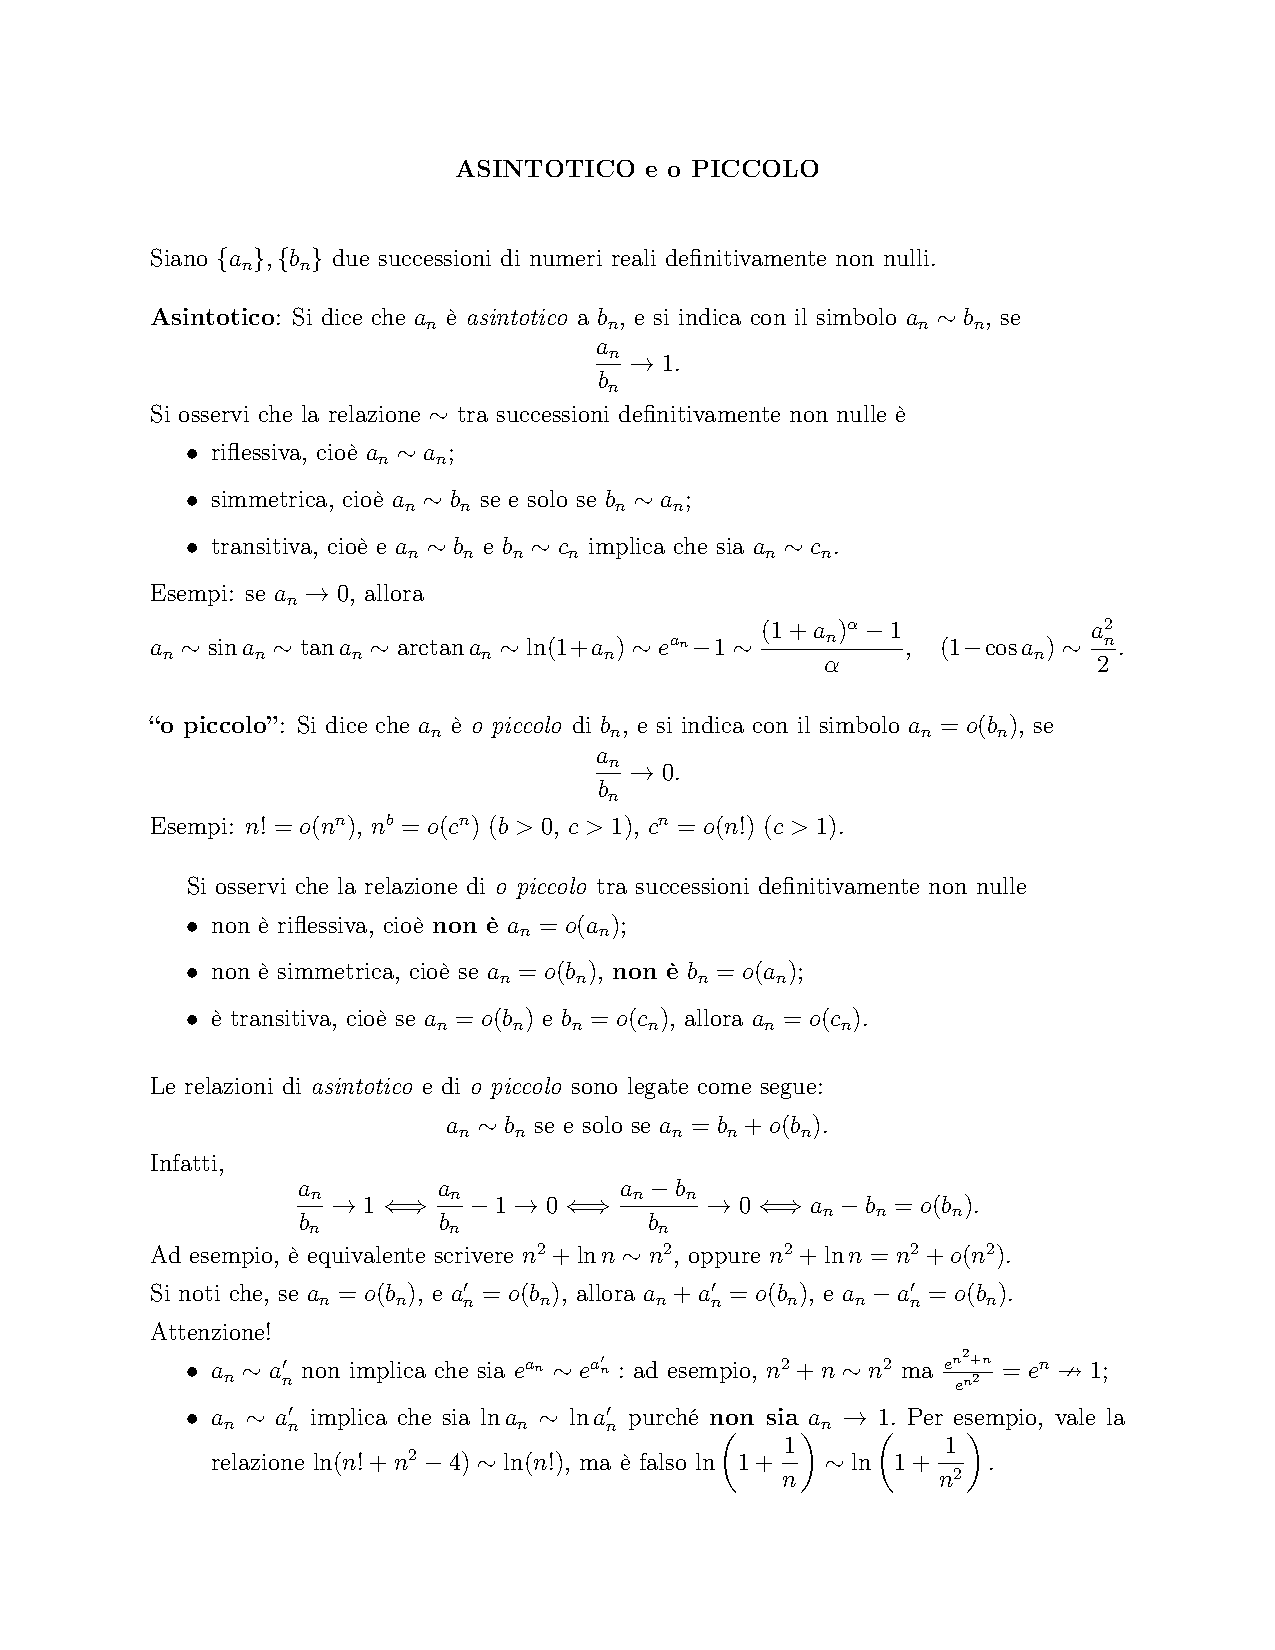
\includepdf[pages=-,pagecommand={},width=1.3\textwidth]{landau.pdf}\end{center}
\section{Limiti Notevoli}
\subsection{Numero di Nepero}
Si introduce, \textit{senza dimostrazione}, uno dei principali limiti notevoli:
$$\lim_{n\rightarrow +\infty}{\left(1+ \frac{1}{n}\right)}^n = e = \mbox{ numero di Nepero}$$ 
Si osserva, di conseguenza, che:
$$\forall\{a_n\} \mbox{, } a_n\rightarrow 0 \mbox{, } a_n\neq 0 \longrightarrow {(1+a_n)}^{\frac{1}{a_n}}\rightarrow e$$
e anche che:
$$\forall\{a_n\} \mbox{, } |a_n|\rightarrow +\infty  \longrightarrow {\left(1+\frac{1}{a_n}\right)}^{a_n}\rightarrow e$$
\subsubsection{Limiti notevoli derivati dal limite notevole di $e$}
Da questo limite notevole si derivano altri limiti notevoli:
\begin{itemize}
\item $a_n\rightarrow 0 \longrightarrow \frac{\ln(1+a_n)}{a_n}\rightarrow 1 \longleftrightarrow \ln(1+a_n)\sim a_n \mbox{ }(\mbox{che si dimostra con ln a }{(1+a_n)}^{\frac{1}{a_n}})$
\item $a_n\rightarrow 0 \longrightarrow \frac{{e}^{a_n}-1}{a_n}\rightarrow 1 \longleftrightarrow {e}^{a_n}-1 \sim a_n$
\item $a_n\rightarrow 0 \longrightarrow \frac{{(1+a_n)}^{\alpha}-1}{a_n}\rightarrow \alpha \longleftrightarrow {(1+a_n)}^{\alpha}-1\sim \alpha\cdot a_n$
\end{itemize}
\subsection{Limite notevole del seno}
Abbiamo inoltre un altro limite notevole molto importante:
$$\mbox{Sia }a_n>0 \mbox{ e } a_n\rightarrow 0 \longrightarrow \frac{\sin {a_n}}{a_n}\rightarrow 1 \longleftrightarrow \sin{a_n}\sim a_n$$
\begin{proof}
Sappiamo che $$\sin{a_n}<a_n<\tan{a_n}$$\\
Passando ai reciproci si ha $$\frac{\cos{a_n}}{sin{a_n}}<\frac{1}{a_n}<\frac{1}{\sin{a_n}}$$
Moltiplicando tutto per $\sin{a_n}$ si ottiene $$\cos{a_n}<\frac{\sin{a_n}}{a_n}<1$$
Sapendo infine che per $a_n\rightarrow 0 \longrightarrow \cos{a_n}\rightarrow 1$ si ottiene $$1<\frac{\sin{a_n}}{a_n}<1$$
e quindi per il teorema del confronto si ha: $$\frac{\sin{a_n}}{a_n} \rightarrow 1$$
\end{proof}
\subsubsection{Limiti notevoli derivati dal limite notevole del seno}
Da questo limite notevole si ricavano i seguenti:
\begin{itemize}
\item $a_n\rightarrow 0 \longrightarrow \frac{\tan{a_n}}{a_n}\rightarrow 1 \longleftrightarrow \tan{a_n}\sim a_n$
\item $a_n\rightarrow 0 \longrightarrow \frac{\arctan{a_n}}{a_n}\rightarrow 1 \longleftrightarrow \arctan{a_n}\sim a_n$
\item $a_n\rightarrow 0 \longrightarrow \frac{1-\cos{a_n}}{{a_n}^{2}}\rightarrow \frac{1}{2} \longleftrightarrow 1-\cos{a_n}\sim \frac{{a_n}^{2}}{2}$
\end{itemize}
\begin{proof}(dell'ultimo limite notevole derivato)\\
Si sa che $$(1-\cos{a_n})\cdot(1+\cos{a_n})=\sin^2{a_n}$$
Grazie al limite notevole $\frac{\sin{a_n}}{a_n} \rightarrow 1$ si ha che $$\frac{\sin^2{a_n}}{{a_n}^{2}} \rightarrow 1.$$
Possiamo quindi dire che: $$\frac{(1-\cos{a_n})\cdot(1+\cos{a_n})}{{a_n}^{2}}\rightarrow 1$$
Essendo inoltre $$(1+\cos{a_n})=2 \mbox{ con } a_n\rightarrow 0$$
Si ottiene $$\frac{(1-\cos{a_n})\cdot 2}{{a_n}^{2}}\rightarrow 1 \longleftrightarrow \frac{1-\cos{a_n}}{{a_n}^{2}}\rightarrow \frac{1}{2} $$
\end{proof}

\chapter{Serie}
Sia $\{a_n\}$ una successione a valori reali. Si costruisce una successione che è la somma dei termini di $a_n$ da $1$ a $k$:
$$\sum_{n=1}^{k}a_n$$ 
questa è una \textit{serie numerica} di termine generale $a_n$.
In altre parole una \textit{serie numerica} è una successione di somme parziali. Si usa la notazione:$$\sum_{n=1}^{+\infty} a_n = a_1+a_2+...+a_n$$
Di una serie solitamente si studia la convergenza o la divergenza. 
\begin{shaded}
\section{Principio di Induzione}
Sia $P(n)$ una proprietà che valga per l'intero $n$. Se $P(n_0)$ è vera e se si suppone $P(n)$ vera allora $P(n+1)$ è vera.\\
\begin{esempio}
Somma dei primi $n$ numeri interi:
\begin{equation}
\sum_{i=1}^{n} i=\frac{n(n+1)}{2}
\end{equation}
\begin{proof}
Si ha, per il \textit{Principio di Induzione} che: $$ \sum_{i=1}^{n+1} i= \frac{(n+1)(n+2)}{2}$$ $$ \sum_{i=1}^{n} i+(n+1) = \frac{n(n+1)+2(n+1)}{2}=\frac{(n+1)(n+2)}{2}= \frac{n(n+1)}{2}+(n+1)$$ $$\mbox{ la tesi è verificata} \rightarrow P(n) \mbox{ è vera } \forall n$$
\end{proof}
\end{esempio}
\end{shaded}
\section{Serie conosciute}
\subsection{Serie geometrica}
$$\overbrace{\sum_{n=0}^{+\infty} q^{n}}^{q\in \mathbb{R}}$$
$$\left\{
\begin{array}{ll}
	\frac{1}{1-q} & \mbox{ } |q|<1\\
	+\infty & \mbox{ } q\geq 1\\
	\mbox{oscilla } & \mbox{ } q\leq -1
\end{array}
\right.$$
\begin{proof}
Questa serie si può definire come:$$A_k=\sum_{n=0}^{k}q^n=1+q+q^2+\cdots+q^k=\frac{1-q^{k+1}}{1-q}$$
Quindi con $|q|<1$ si ha che $q^{k+1}\rightarrow 0$ e la serie converge a $\frac{1}{q+1}$, con $q>1$ si ha che diverge mentre con $q<-1$ si ha un oscillazione tra $+\infty$ e $-\infty$. In caso si $q=1$ si ha banalmente una somma infinita di $1$, quindi diverge.
\end{proof}
\newpage
\subsection{Serie di Mengoli (o Telescopica)}
$$\sum_{n=1}^{+\infty} \frac{1}{n(n+1)} = 1$$
\begin{proof}
Si ha che si può effettuare la seguente scomposizione di $\frac{1}{n(n+1)}$:
$$\frac{A}{n}+\frac{B}{n+1}=\frac{An+A+Bn}{n(n+1)}$$
Dato che $An+A+Bn \overbrace{=}^{!} 1$ si ha:
				$$\left\{
                \begin{array}{ll}
                  A+B=0\\
                  A=1\\
                  B=-1
				\end{array}
				\right.$$
e quindi: $$\frac{1}{n(n+1)}=\frac{1}{n}-\frac{1}{n+1}$$
Se si prova a fare la somma al crescere di $n$ si ha:$$s_n=1-\frac{1}{2}+\frac{1}{2}-\frac{1}{3}+...+\frac{1}{n}-\frac{1}{n+1}=1-\frac{1}{n+1}=1$$
\end{proof} 
\subsection{Serie Armonica}
$$\sum_{n=1}^{+\infty} \frac{1}{n} \mbox{ diverge}$$
\begin{proof}
Considero $$\sum_{n=k}^{2k}\frac{1}{n}=\frac{1}{k}+\frac{1}{k+1}+\frac{1}{k+2}+\cdots+\frac{1}{2k}$$
Poichè il termine generale è monotono decrescente è tutta sicuramente maggiore di $\frac{1}{2k}$, l'ultimo addendo, moltiplicato $k$ volte. Quindi:
$$\frac{1}{k}+\frac{1}{k+1}+\frac{1}{k+2}+\cdots+\frac{1}{2k}>\frac{1}{2k}\cdot k=	\frac{1}{2}$$
Cauchy non è rispettato quindi e la serie diverge.
\end{proof}
\section{Condizione necessaria di convergenza}
\begin{teorema}
Sia $\sum_{n=1}^{+\infty} a_n$ convergente (ovvero che tende ad un numero finito) allora $a_n$  tende a $0$.
\end{teorema}
\begin{proof}
Sia ${\{S_n\}}_{n=1}^{+\infty}$ la successione associata alla serie, allora se la serie converge, per ipotesi, si ha:
$$s_n \rightarrow L\in \mathbb{R}$$
$$s_{n-1} \rightarrow L\in \mathbb{R}$$
$$\downarrow$$
$$s_n-s_{n-1}=a_n\rightarrow L-L\rightarrow 0 \longrightarrow a_n \rightarrow 0$$
\begin{center}in quanto $s_n=s_{n-1}+a_n$.\end{center} 
\end{proof}
\begin{nota}
Se $a_n\not\rightarrow 0$ allora $\sum_{n=1}^{+\infty} a_n$  non converge, ma è \textbf{divergente o indeterminata}.
\end{nota}
\begin{nota}
Non vale il viceversa: se so solo che $a_n\rightarrow 0$, non posso dire nulla sul carattere della serie.
\end{nota}


\section{Operazioni tra Serie}
\begin{itemize}
\item siano $\sum_{n=1}^{+\infty} a_n$ e $\sum_{n=1}^{+\infty} b_n$ due serie convergenti $\longrightarrow$ $\sum_{n=1}^{+\infty} (a_n+b_n)$ converge
\item sia $\sum_{n=1}^{+\infty} a_n$, convergente, e sia $k\in \mathbb{R} \longrightarrow \sum_{n=1}^{+\infty} (k\cdot a_n)=k\cdot \sum_{n=1}^{+\infty} a_n$ converge
\item se $a_n=b_n$ definitivamente allora $\sum_{n=1}^{+\infty} a_n$ e $\sum_{n=1}^{+\infty} b_n$ hanno lo stesso carattere
\end{itemize}

\begin{teorema}
Sia $\sum_{n=1}^{+\infty} a_n$ con $a_n\geq 0$ definitivamente $\forall n\in \mathbb{N}$ allora la serie non può oscillare ma è regolare (quindi converge o diverge a $+\infty$)
\end{teorema}
\begin{proof}
Poiché ogni volta aggiungo alle somme parziali un qualcosa di positivo si ha: $s_n\leq s_{n+1},\mbox{ } \forall n\in \mathbb{N}$; si ha quindi, per il teorema sulle successioni monotone, una successione monotona \textit{Non Decrescente} e quindi si ha sempre un limite (o $+\infty$ o $L\in \mathbb{R}$) e non può oscillare. Stesso vale se la successione fosse monotona decrescente (solo che in caso si avrebbe il limite a $-\infty$ e non a $+\infty$)
\end{proof}
\section{Strumenti per lo studio del Carattere di una Serie}
\subsection{Teorema del confronto per serie numeriche}
\begin{teorema}[del Confronto per Serie Numeriche]
Siano $\sum_{n=1}^{+\infty} a_n$ e $\sum_{n=1}^{+\infty} b_n$, con $0\leq a_n\leq b_n \mbox{ , } \forall n\in \mathbb{N}$ allora:
\begin{itemize}
\item se  $\sum_{n=1}^{+\infty} b_n$ converge (definito maggiorante dell'altra successione) anche $\sum_{n=1}^{+\infty} a_n$ converge.
\item Se $\sum_{n=1}^{+\infty} a_n$ diverge allora anche $\sum_{n=1}^{+\infty} b_n$ diverge.
\end{itemize}
\end{teorema}
\begin{proof}
Si procede così:
\begin{itemize}
\item Si ha, $\forall n\in \mathbb{N}$:
$$\{S_n\}=a_1+...+a_n\leq b_1+...+b_n=\{S^{'}_n\}$$
Suppongo che $s^{'}_n\rightarrow L^{'} \in \mathbb{R}$. Sappiamo che $\{S_n\}$ (supposta monotona \textit{non decrescente}), ammette limite, per la monotonia, ed è limitata; $L^{'}$ è il \textit{sup} di $\{S^{'}_n\}$ ed è maggiorante di $S_n$; quindi si ha:
$$S_n\leq L^{'}, \forall n\mbox{  quindi  } S_n\rightarrow L\in \mathbb{R}\mbox{  finito  } (L<L^{'}) \longrightarrow S_n \mbox{ converge}$$
\item suppongo $s_n\rightarrow +\infty$, \textit{monotona crescente}, e $s^{'}_n\geq s_n$ allora per il \textit{Teorema del confronto} $s^{'}_n$ diverge a $+\infty$
\end{itemize}
\end{proof}
\subsection{Teorema del confronto asintotico}
\begin{teorema}[del Confronto Asintotico]
Siano $\sum_{n=1}^{+\infty} a_n$ e $\sum_{n=1}^{+\infty} b_n$, con $a_n,b_n>0$ e $a_n\sim b_n \mbox{ quindi } \frac{a_n}{b_n}\rightarrow 1$, allora le due serie hanno lo stesso carattere.
\end{teorema}
\begin{proof}
Scelgo un un $\epsilon$ piccolo a piacere, per comodità scelgo $\epsilon=\frac{1}{2}$; allora:
$$\exists n\geq n_0\longrightarrow 1-\epsilon<\frac{a_n}{b_n}<1+\epsilon$$
$$\downarrow$$
$$\mbox{se  } \epsilon=\frac{1}{2}\longrightarrow \frac{1}{2}<\frac{a_n}{b_n}<\frac{3}{2}$$
$$\downarrow$$
$$\frac{b_n}{2}<a_n<\frac{3}{2}\cdot b_n$$
Quindi:
\begin{itemize}
\item se $\sum_{n=1}^{+\infty} a_n$ converge allora $\sum_{n=1}^{+\infty} \frac{b_n}{2} = \frac{1}{2}\sum_{n=1}^{+\infty} b_n$ converge per il \textit{Teorema del confronto} (anche se è moltiplicata per $\frac{1}{2}$ converge, ovviamente)
\item se $\sum_{n=1}^{+\infty} a_n$ diverge allora $\sum_{n=1}^{+\infty} \frac{3}{2}\cdot b_n = \frac{3}{2}\sum_{n=1}^{+\infty} b_n$ diverge per il \textit{Teorema del confronto} (anche se è moltiplicata per $\frac{3}{2}$ diverge, ovviamente)
\end{itemize}
\end{proof}
\subsection{Teorema di condensazione}
\begin{teorema}[Criterio di Condensazione]
Sia $\sum_{n=1}^{+\infty} a_n$ con $a_n>0$ e $a_n\geq a_{n+1}$, successione monotona \textit{decrescente} allora:
$$\sum_{n=1}^{+\infty} a_n \mbox{  e  } \sum_{n=1}^{+\infty} 2^n\cdot a_{2^n} \mbox{  hanno lo stesso carattere}$$
\end{teorema}
Da questo teorema possiamo trarre la seguente applicazione:
\begin{center}
 $\sum_{n=1}^{+\infty} \frac{1}{n^a}=\left\{
                \begin{array}{ll}
                \mbox{Converge con  } \mbox{ } a\geq 2 & \mbox{  in quanto  }\frac{1}{n^a}\leq \frac{1}{n^2}\\
                \mbox{Converge con  } \mbox{ } 1<a<2 & \mbox{  per il Criterio di Condensazione}\\
                \mbox{Diverge con   } \mbox{ } \mbox{ } \mbox{ } 0<a\leq 1 & \mbox{  in quanto  }\frac{1}{n^a}\geq \frac{1}{n}
				\end{array}
				\right.$
\end{center}
Si dice che $\sum_{n=1}^{+\infty} a_n$ \textit{Converge Assolutamente} se $\sum_{n=1}^{+\infty} |a_n|$ converge
\subsection{Teorema della convergenza assoluta}
\begin{teorema}[della Convergenza Assoluta]
Sia $\sum_{n=1}^{+\infty} a_n$, se la serie converge assolutamente allora converge anche semplicemente.
\end{teorema}
\begin{proof}
Sia $a_n=b_n-c_n$  con:
\begin{center}
 $b_n=\left\{                                        
                \begin{array}{ll}						
                a_n & \mbox{ se }  a_n\geq 0\\				
              	0 & \mbox{ se }  a_n< 0					
				\end{array}								
				\right.$										
$c_n=\left\{                                        
                \begin{array}{ll}						
                -a_n & \mbox{ se }  a_n< 0\\				
              	0 & \mbox{ se }  a_n\geq 0					
				\end{array}								
				\right.$		
\end{center}
Si ha quindi:
$$0\leq b_n \leq |a_n| \mbox{  e  } 0\leq c_n \leq |a_n|$$
Per ipotesi $\sum_{n=1}^{+\infty} |a_n|$ converge quindi per il \textit{Teorema del Confronto }anche $b_n$ e $c_n$ convergono:
$$\sum_{n=1}^{+\infty} |a_n|=\sum_{n=1}^{+\infty} (b_n-c_n)=\sum_{n=1}^{+\infty} b_n - \sum_{n=1}^{+\infty} c_n$$
Dove tutti gli elementi di questa equazione convergono, imponendo la convergenza, per conseguenza, da destra a sinistra
\end{proof}
\subsection{Teorema della Radice}
\begin{teorema}[Criterio della Radice]
Sia $\sum_{n=1}^{+\infty} a_n$ , con $a_n>0$ allora:
\begin{center}
 $\sqrt[n]{a_n}=L\in \mathbb{R}=\left\{
                \begin{array}{ll}
                \mbox{se  } L>1 & \mbox{  la serie diverge}\\
                \mbox{se  } (0<)L<1 & \mbox{  la serie converge}\\
                \mbox{se  } L=1 & \mbox{  non si può dire nulla sul carattere della serie}
				\end{array}
				\right.$
\end{center}
\end{teorema}
\begin{proof}
\begin{itemize}
\item sia $(0<)L<1$ e sia $\epsilon >0$ piccolo a piacere. Sia $L+\epsilon<1$; $\exists n\in\mathbb{N} \mbox{  tale che  } \forall n>n_0\mbox{  (definitivamente) }:$
$$\sqrt[n]{a_n}<L+\epsilon \longrightarrow a_n<{(L+\epsilon)}^{n}$$
Dato che ${(L+\epsilon)}^{n}$ è una serie geometrica con $q<1$ converge, quindi anche $a_n$ converge
\item sia $L>1$; tutti i termini di $a_n$ sono maggiori di 1. Ne consegue che:
 $$\sqrt[n]{a_n}>1 \longrightarrow a_n\rightarrow 1$$
\end{itemize}
\end{proof}
\newpage
\subsection{Teorema del rapporto}
\begin{teorema}
Sia $\sum_{n=1}^{+\infty}a_n$ una serie  termini positivi. Supponendo che $\exists \lim_{n\rightarrow +\infty}\frac{a_{n+1}}{a_n}\equiv\alpha$:
\begin{itemize}
\item se $\alpha<1$ la serie converge
\item se $\alpha>1$ la serie diverge e inoltre $a_n\rightarrow +\infty$
\end{itemize}
\end{teorema}
\begin{proof}
\begin{itemize}
Si hanno le dimostrazioni dei due punti:
\item Sia $0<\alpha<1$. Si può definire un $q\in(\alpha,1)$ per cui $\exists N:\forall n>N$ si ha $\frac{a_{n+1}}{a_n}<q$. Allora per questi $n$ si ha:
$$a_n=\frac{a_n}{a_{n-1}}\cdot a_{n-1}=\frac{a_n}{a_{n-1}}\cdot\frac{a_{n-1}}{a_{n-2}}\cdot\frac{a_{n-2}}{a_{n-3}}\cdot\cdots\cdot\frac{a_{N+1}}{a_{N}}\cdot a_N$$
Tutti questi rapporti, del tipo $\frac{a_{k}}{a_{k-1}}$, sono minori di $q$ e quindi:
$$a_n\leq q^n\cdot \frac{a_N}{q^N}$$
Dove $q^n$ è una serie geometrica di ragione minore di 1 ($q<1$), e quindi converge, e quindi, per il teorema del confronto, anche $a_n$ converge.
\item Sia $\alpha>1$. Si può definire un $q\in(1,\alpha)$ per cui $\exists N:\forall n>N$ si ha $\frac{a_{n+1}}{a_n}>q$. Allora per questi $n$ si ha esattamente come sopr, solo che alla fine si ha, perchè tutti i termini sono maggiori di $q$:
$$a_n\geq q^n\cdot \frac{a_N}{q^N}$$
Dove $q^n$ è una serie geometrica di ragione maggiore di 1 ($q>1$), e quindi diverge, e quindi, per il teorema del confronto, anche $a_n$ diverge.
\end{itemize}
\end{proof}
\subsection{Serie conosciute}
Sia $\sum_{n=1}^{+\infty} \frac{1}{n^a}$. essa si risolve con il confronto asintotico il più delle volte.
\begin{center}
 $\sum_{n=1}^{+\infty} \frac{1}{n^a}=\left\{
                \begin{array}{ll}
                \mbox{Converge con  } \mbox{ } a>1 \\
                \mbox{Diverge con   } \mbox{ } \mbox{ } \mbox{ } a\leq 1 
				\end{array}
				\right.$
\end{center}
\begin{esempio}
$$\sum_{n=0}^{+\infty} 2^m\cdot a_{2^m}= \sum_{n=0}^{+\infty} 2^m \cdot \frac{1}{{(2^m)}^a}=\sum_{n=0}^{+\infty} {\left(\frac{1}{{2}^{a-1}}\right)}^m$$
\end{esempio}
\begin{esempio}
Sia data $\sum_{n=2}^{+\infty} \frac{1}{n^a\cdot \log^{b} n}$ si ha:
\begin{center}
 $\sum_{n=2}^{+\infty} \frac{1}{n^a\cdot \log^{b} n}=\left\{
                \begin{array}{ll}
                \mbox{Converge con  } \mbox{ } a>1, \forall b \\
                \mbox{Converge con  } \mbox{ } a=1,b>1\\
                \mbox{Diverge negli altri casi}
				\end{array}
				\right.$
\end{center}
\end{esempio}
Sia $\sum_{n=1}^{+\infty} a_n$ \textit{di segno qualsiasi}. Se  $\sum_{n=1}^{+\infty} |a_n|$ converge anche la serie iniziale converge
\begin{esempio} 
\begin{itemize}
\item $\sum_{n=1}^{+\infty} \frac{(-1)^n}{n^2}\sim \sum_{n=1}^{+\infty} \frac{1}{n^2}  \mbox{ converge per convergenza assoluta}$
\item $\sum_{n=1}^{+\infty} \frac{(-1)^n}{n}\sim \sum_{n=1}^{+\infty} \frac{1}{n}  \mbox{ non si può dire nulla sulla divergenza assoluta}$
\item $\sum_{n=1}^{+\infty} \frac{(\sin{n})}{n} \mbox{ non sappiamo dire nulla}$
\end{itemize}
\end{esempio}
\subsection{Criterio di Leibniz}
\begin{teorema}[criterio di Leibniz]
Sia $$\sum_{n=1}^{+\infty} (-1)^{n+1}\cdot a_n$$. Si ha una serie oscillante. Se:
\begin{itemize}
\item $a_n \geq 0$
\item $a_n \geq a_{n+1}$
\item $a_n\rightarrow 0$
\end{itemize}
allora la serie converge
\end{teorema}
\begin{proof}
Si ha: $s_1=a_1, \mbox{ } s_2=a_1-a_2,\mbox{ } s3=a_1-a_2+a_3 \mbox{ ovvero } (s_2+a_3), ...$\\ Quindi $\{s_{2n}\}$, le successioni delle somme parziali di indici pari, è monotona \textit{non decrescente} e superiormente limitata. Quindi $$s_{2n}\rightarrow S\in \mathbb{R}$$
$$\exists \epsilon >0, \mbox{ } \exists n_0, \forall n\geq n_0 \longrightarrow S-\epsilon<s_{2n}\leq S$$
Vediamo le somme parziali di indice dispari. Dato che $a_n\rightarrow 0$ $$\exists \overline{N}, \forall n\geq \overline{n} \longrightarrow a_n<\epsilon$$
Quindi:$$ s_{2n}+a_{2n+1}<S+\epsilon$$
In conclusione $\forall n$
$$S-\epsilon<s_{2n}+s_{2n+1}<S+\epsilon$$ 
Quindi la successione delle somme parziali ammette limite finito
\end{proof}
\begin{esempio}
\begin{itemize}
\item $$\sum_{n=1}^{+\infty} \frac{(-1)^n}{n}$$ Si ha: $\frac{1}{n}>\frac{1}{n+1}$ e $\frac{1}{n}\rightarrow 0$. Quindi la serie converge.
\item $$\sum_{n=1}^{+\infty} \frac{(-1)^n}{n-\sqrt{n}}$$ Si ha: $$n-\sqrt{n}\leq n+1 - \sqrt{n+1}$$ e quindi: $$\sqrt{n+1}\leq n+\sqrt{n}$$ infine: $$\sqrt{n+1}\leq 1+n+2 \cdot \sqrt{n}$$
\end{itemize}
\end{esempio}
\subsection{Teorema di Dirichlet}
\begin{teorema}[di Dirichlet]
Sia $\sum_{n=1}^{+\infty} a_n$ una serie assolutamente convergente. Allora, per ogni permutazione $\pi:\mathbb{N}\rightarrow \mathbb{N}$ si ha che la serie $\sum_{n=1}^{+\infty} a_{\pi (n)}$ è convergente alla stessa somma. (Attenzione: deve essere una convergenza assoluta)
\end{teorema}

\chapter{Funzioni}
Si definisce una funzione $f$ come:
$$f:D\subseteq \mathbb{R}\rightarrow \mathbb{R}$$
In generale con $D=(a,b)$  o $D=(a,b)\cup(c,d)$.\\
Per calcolare il limite di una funzione lo si calcola nei \textit{punti di accumulazione}.
\begin{definizione}
Sia $f:D\subseteq \mathbb{R}\rightarrow \mathbb{R}$ e sia $x_0\in D^{'}$ ($D^{'}$ indica l'insieme dei punti di accumulazione di $D$). Si dice che:
$$\lim_{x\rightarrow x_0} f(x)=L, \mbox{ con } L\in \mathbb{R}$$
se: $$\forall \epsilon>0, \mbox{  } \exists\delta>0: \mbox{  } \forall x\in B(x_0,\delta)\backslash\{x_0\} \mbox{  si ha  } f(x)\in B(L,\epsilon)$$
Cioè se:
$$|x-x_0|<\delta, \mbox{ con } x\neq x_0 \mbox{ e } x\in D, \mbox{ comporta } |f(x)-L|<\epsilon$$
\end{definizione}
\begin{definizione}
Si dice che: 
$$\lim_{x\rightarrow x_0} f(x) = +\infty$$ 
se:
$$\forall k\in \mathbb{R}, \mbox{ } \exists \delta>0:\mbox{ } \forall x\in B(x_0,\delta)\backslash\{x_0\} \mbox{  si ha  } f(x)>k$$
Se il limite di $f(x)$ diverge ( a $+\infty$ o $-\infty$) la retta $x=x_0$ si dice \textbf{Asintoto Verticale} per $f$.
\end{definizione}
\newpage
\begin{definizione}
Sia $+\infty$ punto di accumulazione per $D$ (ovvero $D$ non è superiormente limitato). Si dice che:
$$\lim_{x\rightarrow +\infty} f(x) =L, \mbox{ con } L\in\mathbb{R}$$
se:
$$\forall \epsilon>0, \mbox{  } \exists M\in \mathbb{R}, \mbox{  }\forall x\in(M,+\infty) \mbox{ e } x\in D, \mbox{ tale che } f(x)\in B(L,\epsilon)$$
Se il limite di $f(x)$ tende a $L\in\mathbb{R}$ la retta $y=L$ si chiama \textbf{Asintoto Orizzontale} per $f$ (vale sia con $x\rightarrow +\infty$ che con $x\rightarrow -\infty$)
\end{definizione}
\begin{definizione}
Si dice che:
$$\lim_{x\rightarrow +\infty} f(x) = +\infty$$ 
se:
$$\forall k\in \mathbb{R}, \mbox{ } \exists  H\in \mathbb{R}: \mbox{ } \forall x\in(H,+\infty), \mbox{ con } x\in D, \mbox{ si ha } f(x)\in (k,+\infty)$$
\end{definizione}
\begin{definizione}
Sia $f:\mathbb{R}\rightarrow \mathbb{R}$, $f$ periodica con periodo $T$( cioè $T$ è il più piccolo numero positivo , $\neq 0$, tale che $f(x+T)=f(x), \mbox{ } \forall x\in \mathbb{R}$).
Se:
$$\lim_{x\rightarrow +\infty}f(c)=L, \mbox{ con } L\in\mathbb{R}, \mbox{ allora } f(x)=L \mbox{ } \forall x\in\mathbb{R}$$
\begin{proof}
Sia per assurdo $f$ non costante, cioè: 
$$\exists x_0\in\mathbb{R}: \mbox{ } f(x_0)=L^{'}\neq L$$
%sistemare questa dimostrazione
\end{proof}
\end{definizione}
\begin{definizione}
Sia $f:D\rightarrow R$, con $x_0$ punto di accumulazione di $D$. Si dice che:
$$\lim_{x\rightarrow x^{-}}f(x)=L, +\infty, -\infty$$
se, per ogni intorno di $L$ o di $+\infty$ o di $-\infty$:
$$\exists\delta>0: \mbox{ } \forall x\in (x_0-\delta,x_0) \mbox{ si ha l'esistenza del limite}$$
%sistemare questa definzione
\end{definizione}
\subsubsection{Teorema di collegamento}
\begin{teorema}[di collegamento]
Sia $f:D\rightarrow \mathbb{R}$ sia $p\in \mathbb{R}^{*}$ punto di accumulazione per $D$. Allora:
$$\lim_{x\rightarrow p}f(x)=L, \mbox{ } L\in \mathbb{R}^{*}, \mbox{ sse } \forall \{x_n\}\subset D, \mbox{ con } x_n\neq p \mbox{ e } x_n\rightarrow p, \mbox{ si ha } f(x_n)\rightarrow L$$
\end{teorema}
\begin{esempio}
\begin{itemize}
Due esempi di applicazione:
\item Applico il teorema del collegamento a $\frac{sin (x) }{x}$. Dato che:
$$\lim_{x\rightarrow 0} \frac{sin (x)}{x}=1 \mbox{ si ha: } \lim_{n\rightarrow +\infty}\frac{sin (a_n)}{a_n}=1, \forall \{a_n\}\rightarrow 0,\,\{a_n\}\neq 0$$
\item Posso dimostare che: $$\nexists  \lim_{x\rightarrow +\infty} sin\left(\frac{1}{x}\right)$$
in quanto posso definire $\frac{1}{x}=\pi\cdot n$, avendo quindi sempre un argomento del $sin$ che diverge, in questo caso:
$$\lim_{x\rightarrow +\infty} sin\left(\pi\cdot n\right)=0$$
posso però anche definire $\frac{1}{x}=\frac{\pi}{2}\cdot n$, che diverge comunque però:
$$\lim_{x\rightarrow +\infty} sin\left(\frac{\pi}{2}\cdot n\right)=0,1,-1\mbox{ (oscilla)}$$
Si ha quindi che non tutte le sottosuccessioni hanno lo stesso limite, quindi il teorema del collegamento garantisce l'inesistenza del limite.
\end{itemize}
\end{esempio}
\begin{shaded}
\begin{osservazione}
Se $$\lim_{x\rightarrow x_0} f(x)$$ è unico lo sono anche:
$$\lim_{x\rightarrow x_0^{-}} f(x)=L$$
$$\lim_{x\rightarrow x_0^{+}} f(x)=L$$
\end{osservazione}
\begin{osservazione}
sia $x_0$ di accumulazione per $D$ sia \textit{a sinistra (-)} che \textit{a destra (+)} allora:
$$\lim_{x\rightarrow x_0} f(x)=L$$ sse:
$$\lim_{x\rightarrow x_0^{+}} f(x)=L$$ e
$$\lim_{x\rightarrow x_0^{-}} f(x)=L$$
comodo per calcolare limiti verso un punto non incluso nel dominio.
\end{osservazione}
\end{shaded}
\subsubsection{Teorema di unicità del limite}
\begin{teorema}
Sia $f:D\rightarrow \mathbb{R}$ e $p\in\overline{\mathbb{R}}$ punto di accumulazione per $D$. Se:
$$\exists \lim_{x\rightarrow p}f(x)=L,\,L\in\overline{\mathbb{R}}$$
allora questo limite è unico.
\end{teorema}
\subsubsection{Teorema di permanenza del segno}
\begin{teorema}[di permanenza del segno]
Sia $f:D\rightarrow \mathbb{R}$ e $p, \in \overline{\mathbb{R}}$ di accumulazione per $D$. Se:
$$\lim_{x\rightarrow p} f(x)>0$$
allora $f(x)>0$ $\forall x$ in un opportuno intorno di $p$ (e in $D$).
\end{teorema}
\subsubsection{Teorema del confronto}
\begin{teorema}[del confronto]
Siano $f,g,h:D\rightarrow \mathbb{R}$ e $p$ di accumulazione per $D$. Se:
\begin{itemize}
\item $f(x)\leq g(x)\leq h(x),\mbox{ } \forall x\in D \backslash \{p\}$
\item $\lim_{x\rightarrow p} f(x) =\lim_{x\rightarrow p} h(x)=L$
\end{itemize}
allora:
 $$\lim_{x\rightarrow p} g(x)=L$$
\end{teorema}
\begin{osservazione}
Se si ha $h(x)\cdot k(x)$ con $h(x)\rightarrow 0, \mbox{ per } x\rightarrow p$ e $|k(x)<c|$, con $c$ costante, allora:
$$0\leq |h(x)\cdot k(x)|\leq |h(x)\cdot c|$$ 
\end{osservazione}
\begin{corollario}
Se $f,g:D\rightarrow \mathbb{R}$, $p$ di accumulazione per $D$. Se
\begin{itemize}
\item $f(x)\leq g(x)$
\item  $$\lim_{x\rightarrow p} f(x) = +\infty$$
\end{itemize}
allora:
$\lim_{x\rightarrow p} g(x) =+\infty$
Vale anche con $-\infty$
\end{corollario}
\begin{nota}
\begin{shaded}
Una funzione $f:D\rightarrow \mathbb{R}$ è una funzione monotona \textit{non decrescente} se:
$$\forall x_1,x_2\in D, \mbox{ } x_1<x_2, \mbox{ si ha } f(x_1)\leq f(x_2)$$
Una funzione $f:D\rightarrow \mathbb{R}$ è una funzione monotona \textit{crescente} se:
$$\forall x_1,x_2\in D, \mbox{ } x_1<x_2, \mbox{ si ha } f(x_1)< f(x_2)$$
Una funzione $f:D\rightarrow \mathbb{R}$ è una funzione monotona \textit{non crescente} se:
$$\forall x_1,x_2\in D, \mbox{ } x_1<x_2, \mbox{ si ha } f(x_1)\geq f(x_2)$$
Una funzione $f:D\rightarrow \mathbb{R}$ è una funzione monotona \textit{decrescente} se:
$$\forall x_1,x_2\in D, \mbox{ } x_1<x_2, \mbox{ si ha } f(x_1)> f(x_2)$$
\end{shaded}
\end{nota}
\begin{teorema}[di esistenza del limite per funzioni monotone]
Sia $f:D\rightarrow \mathbb{R}$, con $D=(a,b)$, se $f$ è monotona \textit{non decrescente} allora:
$$\exists \mbox{ } \lim_{x\rightarrow b^{-}} f(x)$$
e inoltre:
$$ \lim_{x\rightarrow b^{-}} f(x)=\sup\{f(x)\}, \mbox{ con } x\in (a,b)$$
ovviamente:
$$\exists \mbox{ } \lim_{x\rightarrow a^{+}} f(x)$$
e inoltre:
$$ \lim_{x\rightarrow a^{+}} f(x)=\inf\{f(x)\}, \mbox{ con } x\in (a,b)$$
\end{teorema}
\newpage
\begin{shaded}
\begin{nota}[qualche limite importante]
Si hanno:
\begin{enumerate}
\item $f(x)=x^\alpha : (0,+\infty)\rightarrow \mathbb{R}, \mbox{ con }\alpha \in \mathbb{R}$
	\begin{itemize}
	\item $x\rightarrow +\infty=\left\{
                \begin{array}{ll}
                +\infty \mbox{ con } \alpha>0 \\
               	1 \mbox{ con } \alpha=0 \\
                0 \mbox{ con } \alpha<0 \\
				\end{array}
				\right.$
	\item $x\rightarrow 0^{+}=\left\{
                \begin{array}{ll}
                0 \mbox{ con } \alpha>0 \\
               	1 \mbox{ con } \alpha=0 \\
                +\infty \mbox{ con } \alpha<0 \\
				\end{array}
				\right.$
	\end{itemize}
\item $f(x)=\alpha^x : \mathbb{R}\rightarrow \mathbb{R}$
	\begin{itemize}
	\item $x\rightarrow +\infty=\left\{
                \begin{array}{ll}
                +\infty \mbox{ con } \alpha>1 \\
               	1 \mbox{ con } \alpha=1 \\
                0 \mbox{ con } 0<\alpha<1 \\
				\end{array}
				\right.$
	\item $x\rightarrow 0=\left\{
                \begin{array}{ll}
                0 \mbox{ con } \alpha>1 \\
               	1 \mbox{ con } \alpha=1 \\
                +\infty \mbox{ con } 0<\alpha<1 \\
				\end{array}
				\right.$
	\end{itemize}
\item $f(x)=log_\alpha x : (0,+\infty)\rightarrow \mathbb{R}, \mbox{ con } \alpha\neq 1 \mbox{ e } \alpha >0$
\begin{itemize}
	\item $x\rightarrow +\infty=\left\{
                \begin{array}{ll}
                +\infty \mbox{ con } \alpha>1 \\
                -\infty \mbox{ con } 0<\alpha<1 \\
				\end{array}
				\right.$
	\item $x\rightarrow 0=\left\{
                \begin{array}{ll}
                -\infty \mbox{ con } \alpha>1 \\
                +\infty \mbox{ con } 0<\alpha<1 \\
				\end{array}
				\right.$
	\end{itemize}
\end{enumerate}
\end{nota}
\end{shaded}
\newpage
\subsection{Operazioni sui limiti}
\begin{teorema}[dell'algebra dei limiti]
Siano $f,g:D\rightarrow \mathbb{R}$, $p$ di accumulazione per $D$.
Se:
$$\lim_{x\rightarrow p} f(x)=L_1$$
e 
$$\lim_{x\rightarrow p} g(x)=L_2$$
allora:
$$\lim_{x\rightarrow p} (f+g)(x)=L_1+L_2$$
$$\lim_{x\rightarrow p} (f\cdot g)(x)=L_1\cdot L_2$$
$$\lim_{x\rightarrow p} \left(\frac{f}{g}\right)(x)=\frac{L_1}{L_2}$$
Purché le operazioni siano definite in $\overline{\mathbb{R}}$
\end{teorema}
\begin{osservazione}
Se $f(x)\rightarrow L, \mbox{ con } L>0$ e $ g(x)\rightarrow 0$ ma si ha $g(x)>0$ in un intorno di $p\backslash\{p\}$, allora:
$$\lim_{x\rightarrow p} \frac{f(x)}{g(x)}=+\infty$$
\end{osservazione}
\subsubsection{Teorema del limite di composizione}
\begin{teorema}[del limite di composizione]
Siano $f:D_1\rightarrow \mathbb{R}$ e $g:D_2\rightarrow \mathbb{R}$. Sia $p_1$ di accumulazione per $D_1$. Si ha:
$$\lim_{x\rightarrow p_1} f(x)=L_1$$
Si ha poi che $L_1$ è di accumulazione per $D_2$ e quindi:
$$\lim_{t\rightarrow L_1} g(t)=L_2$$
ovvero se:
$$\exists \mbox{ } (g\circ f)(x), \mbox{ } \forall x\in D_2$$
allora:
$$\lim_{x\rightarrow p_1}(g\circ f)(x)=\lim_{x\rightarrow p_1}g(f(x))=\lim_{t\rightarrow L_1}g(t)$$
\end{teorema}
\section{Continuità}
Sia $f:D\rightarrow \mathbb{R}$, sia $x_0\in D$, con $x_0$ di accumulazione per $D$. Si dice che $F$ è continua in $x_0$ se:
$$\lim_{x\rightarrow x_0} f(x)=f(x_0)$$
\begin{teorema}
Le funzioni elementari sono continue in ogni punto del loro dominio.
\end{teorema}
\begin{esempio}
Sia $f(x)=e^x$, con $x_0\in\mathbb{R}_0$:
$$\lim_{x\rightarrow x_0} e^x=e^{x_0}$$
allora $\exists \epsilon>0:\,\exists \delta>0\rightarrow \, \forall x |x-x_0|<\delta\rightarrow \, |e^x-e^{x_0}|<\epsilon$, quindi $e^{x_0}-\epsilon<e^x<e^{x_0}+\epsilon$
Passando hai logaritmi si ha:
$$\log(e^{x_0}-\epsilon)<x<\log(e^{x_0}+\epsilon)\longrightarrow \log(1-\frac{\epsilon}{e^{x_0}})<x-x_0<\log(1+\frac{\epsilon}{e^{x_0}})$$
ponendo $m=\min\{\log(1-\frac{\epsilon}{e^{x_0}},\,\log(1+\frac{\epsilon}{e^{x_0}}\}$ si ha che $|x-x_0|<m\rightarrow \, |e^x-e^{x_0}|<\epsilon$ e quindi si ha continuità in $x_0$
\end{esempio}
\begin{nota}
Se $x_0\in D$ è di accumulazione per $D$ $f$ è:
\begin{itemize}
\item continua \textit{da destra} in $x_0$ se:
$$\lim_{x\rightarrow x_0^{+}} f(x)=f(x_0)$$
\item continua \textit{da sinistra} in $x_0$ se:
$$\lim_{x\rightarrow x_0^{-}} f(x)=f(x_0)$$
\item continua su $D$ se contemporaneamente continua sia \textit{da destra} che \textit{da sinistra}
\end{itemize}
\end{nota}
\newpage
\subsubsection{Teorema di continuità di somma, prodotto e quoziente}
\begin{teorema}[di continuità di somma, prodotto e quoziente]
Siano $f,g:D\rightarrow \mathbb{R}$, $x_o\in D$, punto  di accumulazione per $D$. Se $f$ e $g$ sono continue in $x_0$ lo sono anche:
\begin{itemize}
\item $f+g$
\item $f\cdot g$
\item $\frac{f}{g}$ ( con $g(x)\neq 0$)
\end{itemize}
\end{teorema}
\begin{proof}
\begin{itemize}
\item per $f+g$:
$$\lim_{x\rightarrow x_0} (f+g)(x)=(f+g)(x_0)$$
\begin{center}$\downarrow$ \end{center}
$$\lim_{x\rightarrow x_0} (f(x)+g(x))=\lim_{x\rightarrow x_0} f(x)+\lim_{x\rightarrow x_0} g(x)=f(x_0)+g(x_0)=(f+g)(x_0)$$
\item per $f\cdot g$:
$$\lim_{x\rightarrow x_0} (f\cdot g)(x)=(f\cdot g)(x_0)$$
\begin{center}$\downarrow$ \end{center}
$$\lim_{x\rightarrow x_0} (f(x)\cdot g(x))=\lim_{x\rightarrow x_0} f(x)\cdot \lim_{x\rightarrow x_0} g(x)=f(x_0)\cdot g(x_0)=(f\cdot g)(x_0)$$
\item per $\frac{f}{g}$, con $g(x_0)\neq 0$:
$$\lim_{x\rightarrow x_0} \left(\frac{f}{g}\right)(x)=\left(\frac{f}{g}\right)(x_0)$$
\begin{center}$\downarrow$ \end{center}
$$\lim_{x\rightarrow x_0} \left(\frac{f(x)}{g(x)}\right)=\frac{\lim_{x\rightarrow x_0} f(x)}{\lim_{x\rightarrow x_0} g(x)}=\frac{f(x_0)}{g(x_0)}=\left(\frac{f}{g}\right)(x_0)$$
\end{itemize}
\end{proof}
\begin{definizione}
Si dice che $f$ è continua in $D$ se $f$ è continua in tutti i punti di $D$ 
\end{definizione}
%vedere riga sotto nelle scan ( è la definzione di polinomio)$
\subsubsection{teorema di continuità delle composizioni}
\begin{teorema}[di continuità delle composizioni]
Siano $f:D_1\rightarrow \mathbb{R}$, continua in $x_0$ e $g:D_2\rightarrow \mathbb{R}$, con $f(x_0)\in D_2$ e $g$ continua in $x_0$. Inoltre $\exists g\circ f$ in un intorno di $x_0$. Allora $g\circ f$ è continua in $x_0$
\end{teorema}
\begin{proof}
Sia: 
$$\epsilon >0, \mbox{ } \exists \delta> 0: \mbox { } |x-x_0|<\delta , \mbox{ } x\in  D_1$$
\begin{center}$\downarrow$ \end{center}
$$|(f\circ g)(x)=(f\circ g)(x_0)|<\epsilon \longrightarrow |g(f(x))-g(f(x_0))|<\epsilon$$
Sia ha $\epsilon > 0$, per continuità di $g$:
$$\exists \delta_1>0 \mbox{ } |y-f(x_0)|<\delta_1 \rightarrow |g(y)-g(f(x_0))|<\epsilon$$
Sia ha $\epsilon > 0$, per continuità di $g$:
$$\exists \delta_2>0: \mbox{ } |x-x_0|<\delta_2 \longrightarrow |f(x)-f(x_0)|<\delta_1$$
quindi: 
$$\epsilon\longrightarrow \epsilon>0 \longrightarrow |x-x_0|<\delta_2$$
\begin{center}$\downarrow g$ \end{center}
$$\delta_1 \longrightarrow  \longrightarrow  |f(x)-f(x_0)|<\delta_1$$
\begin{center}$\downarrow f$ \end{center}
$$\delta_2 \longrightarrow  \longrightarrow  |g(f(x))-g(f(x_0))|<\epsilon$$
\end{proof}
\newpage
\subsection{Discontinuità}
Sia $f:D\rightarrow \mathbb{R}$ $x_o\in D$, punto  di accumulazione per $D$. Se $f$ non è continua in $x_0$ si dice \textit{Discontinua} in $x_0$.
Si hanno i seguenti tipi di discontinuità:
\begin{itemize}
\item \textbf{I specie}:
$$\lim_{x\rightarrow x_0} f(x)=L_1, \mbox{ } L_1\in \mathbb{R}$$
$$\lim_{x\rightarrow x_0} f(x)=L_2, \mbox{ } L_2\in \mathbb{R}$$
\begin{center}con\end{center} $$L-1\neq L_2$$
\item \textbf{II specie}:
$$\lim_{x\rightarrow x_0^{+}} f(x) \mbox{ è infinito o non esiste}$$
\begin{center}oppure\end{center}
$$\lim_{x\rightarrow x_0^{-}} f(x) \mbox{ è infinito o non esiste}$$
\item \textbf{III specie (discontinuità \textit{eliminabile})}:
$$\lim_{x\rightarrow x_0} f(x)=L, \mbox{ } L\in \mathbb{R}, \mbox{ con } L\neq f(x_0)$$
\end{itemize}
\subsubsection{Esempi di Continuità}
\begin{itemize}
\item $P_n(x)$, i polinomi sono funzioni continue
\item $\frac{P_n(x)}{Q_n(x)}, \mbox{ } Q_n(x)\neq 0$, le funzioni razionali sono continue
\item $|x|$, il modulo di $x$ è continuo
\item ci sono funzioni, come $\sqrt{\log(\sin x)}$, che sono continue in punti isolati
\item $f(x)=\left\{
                \begin{array}{ll}
                x \mbox{ con } x\in\mathbb{Q} \\
                2x \mbox{ con } x\not\in\mathbb{Q} \\
				\end{array}
				\right.$ è continua solo nell'origine, negli altri punti ha una discontinuità di \textbf{II specie} perché non ho i limiti
\end{itemize}
\newpage
\section{Proprietà delle funzioni continue in intervalli}
Le seguenti proprietà valgono solo se l'insieme è un intervallo
\begin{teorema}[degli zeri]
sia $f:[a,b]\rightarrow \mathbb{R}$, $f$ continua, $f(a)\cdot f(b)\neq 0$ (hanno segno diverso). Allora $\exists x_0\in (a,b) \mbox{ tale che } f(x_0)=0$
\end{teorema}
\begin{proof}
Sia $f(a)<0$ e $f(b)>0$ chiamo $S=\{x\in [a,b]\} \mbox{tale che} f(x)<0$. Tale insieme è:
\begin{itemize}
\item $S \neq \emptyset$ infatti $a\in S$
\item superiormente limitato e $\exists \sup S= x_0$
\end{itemize}
Provo che $x_0$ è zero della funzione: $f(x_0)=0$.\\ Procedo per assurdo, $f(x_0)<0$. In questo caso, per il teorema della permanenza del segno, avremmo  $f(x)<0 \mbox{ } \forall x \in (x_0-\delta, x_0+\delta)$ ma allora $\sup S>x_0$, ma sappiamo che oltre $x_0$ non si può andare, essendo il \textit{sup}.\\
%da guardare
Se $f(x_0)>0$. In questo caso, per il teorema della permanenza del segno, avremmo $f(x)>0 \mbox{ } \forall x \in (x_0-\delta, x_0+\delta)$ e $\inf S<x_0$.\\
Quindi vale $0$ in quel punto. 
\end{proof}
\begin{shaded}
Sia $f$ una funzione qualsiasi, $f:D\rightarrow \mathbb{R}$. $x_0\in D$ è un \textit{punto fisso} se $f(x_0)=x_0$.
\end{shaded}
\subsubsection{Teorema del punto fisso}
\begin{osservazione}[teorema del punto fisso]
Sia $f:[0,1]\rightarrow[0,1]$ continua. Allora esiste punto fisso per $f \in [0,1]$
\begin{proof}
Sia $g(x)=f(x)-x$. Allora:
$g(x)=\left\{
                \begin{array}{ll}
                g(0)=f(0)>0\\
                g(1)=f(1)-1\leq 0\\
				\end{array}
				\right.$\\ Quindi $\exists x_0 \in (0,1) \longrightarrow f(x_0)=x_0$
\end{proof}
\end{osservazione}
\begin{osservazione}[metodo di bisezione]
Sia $f:(a,b)\rightarrow \mathbb{R}$, continua , $f(a)>0$ e  $f(b)<0$
Prendo il punto medio tra gli estremi( $a=\alpha_0, \mbox{ } b=\beta_0$. Se $\frac{\alpha_0+\beta_0}{2}>0$ il nuovo intervallo diventa $[\frac{\alpha_0+\beta_0}{2}=\alpha_1,\beta_0=\beta_1]$ e se $\frac{\alpha_0+\beta_0}{2}<0$  diventa $[\alpha_0=\alpha_1,\frac{\alpha_0+\beta_0}{2}=\beta_1]$. Si ha $[\alpha_0, \beta_0]>[\alpha_1, \beta_1]>...>[\alpha_n, \beta_n]$ Proseguo fino a che ho $\{\alpha_n\}\rightarrow L_1$ e $\{\beta_n\}\rightarrow L_2 $. Dato che $\alpha_n-\beta_n=\frac{b-a}{2^{n}}\rightarrow 0$ allora $L_1=L_2$
\end{osservazione}
%da riguardare
\subsubsection{Teorema di Darboux}
\begin{corollario}[teorema di Darboux o dei valori intermedi]
Sia $f:I\rightarrow \mathbb{R}$, \textit{I} intervallo qualsiasi e $f$ continua in \textit{I}. Allora:
$$ f(I) \mbox{ è un intervallo}$$
\end{corollario}
\begin{proof}
Siano $y_1, y_2 \in f(I)$, $y_1<y_2$, $y_1=f(x_1)$ e $y_2=f(x_2)$. Sia $y_0\in[y_1, y_2]$. Allora:
$$y_0\in f(I)$$
$f(x)-y_0:[x_1,x_2]\rightarrow \mathbb{R} \longrightarrow
\left\{
        \begin{array}{ll} 
        f(x_1)-y_0=y_1-y_0<0\\
        f(x_2)-y_0=y_2-y_0>0\\
        \end{array}
\right.$
\end{proof}
\begin{shaded}
\begin{definizione}
Sia $f:D\rightarrow \mathbb{R}$, $x_0\in D$. 
\begin{itemize}
\item $x_0$ è \textit{punto di massimo assoluto globale per $f$} se $f(x_0)\geq f(x), \mbox{ } \forall x$ 
\item $x_0$ è \textit{punto di minimo assoluto globale per $f$} se $f(x_0)\leq f(x), \mbox{ } \forall x$ 
\item $x_0$ è \textit{punto di massimo assoluto locale per $f$} se $\exists B(x_0,r) \mbox{ tale che }f(x_0)\geq f(x)   \mbox{ } \forall x\in B(x_0,r)\cap D$ 
\item $x_0$ è \textit{punto di minimo assoluto locale per $f$} se $\exists B(x_0,r) \mbox{ tale che }f(x_0)\leq f(x)   \mbox{ } \forall x\in B(x_0,r)\cap D$
\end{itemize}
Una funzione ha massimo se ha un \textit{massimo assoluto globale}, ha invece minimo se ha un \textit{minimo assoluto globale}
\end{definizione}
\end{shaded}
\subsection{Teorema di Weierstrass}
\begin{teorema}[di Weierstrass]
Sia $f:[a,b]\rightarrow \mathbb{R}$, continua. Allora $f$ ha sia massimo che minimo in $[a,b]$.
\end{teorema}
%da riguardare
\begin{nota}
Nel caso di intervalli illimitati si possono trovare massimo e/o minimo globali restringendo l'intervallo ad un insieme limitato e osservando l'andamento della funzione (per esempio $f(x)=x^4+x^3+x^2-1$, che tende a $+\infty$ sia con $x\rightarrow -\infty$ che con $x\rightarrow +\infty$, ha per forza un minimo globale).
\end{nota}
\newpage
Dal seguente teorema e da quello dei valori intermedi si ha, in particolare, che:
\begin{shaded}
\begin{definizione}
$$\mbox{Se } f:[a,b]\rightarrow \mathbb{R} \mbox{, f continua allora:}$$
$$f([a,b])=[m,M] \mbox{ con } m=\mbox{ min f}, \mbox{ e } M=\mbox{ max f}$$
\end{definizione}
\end{shaded}
\subsection{Teorema della funzione inversa}
Se $f:D\rightarrow \mathbb{R}$ se $f$ è \textit{iniettiva}, $f:D\rightarrow Im(f)=f(D)$
Se $f$ è monotona crescente o decrescente (in senso stretto) allora $f$ è \textit{Biunivoca} tra $D$ e $f(D)=Im(f)$
Se $f:D\rightarrow \mathbb{R}$ è \textit{continua} e \textit{iniettiva} allora $f^{-1}:f(D)\rightarrow D$ si può dire questso:
\begin{teorema}[della funzione inversa]
Sia $f:[a,b]\rightarrow \mathbb{R}$, $f$ crescente e strettamente monotona. Allora: $$\exists f^{-1}:\overbrace{[m,M]}^{=Im(f)}\rightarrow [a,b]$$ e $f^{-1}$ è continua.
\end{teorema}
\newpage
\begin{shaded}
\begin{definizione}
Siano $f,g:D\rightarrow \mathbb{R}$ , $p$ di accumulazione per $D$. Sia $g(x)\neq 0$ in un intorno di $p$. Si dice che $f\sim g, \mbox{ per } x\rightarrow p$ se:
$$\lim_{x\rightarrow p} \frac{f(x)}{g(x)}=1$$
\end{definizione}
\subsection{Limiti notevoli per funzioni}
\begin{definizione}
Limiti notevoli per $x\rightarrow 0$
$$\sin x\sim x$$
$$ln(1+x)\sim x$$
$$e^x-1\sim x$$
$$(1+x)^\alpha-1\sim \alpha\cdot x$$
$$\tan x\sim x$$
$$(1-\cos x)\sim \frac{x^2}{2}$$
Valgono anche se si ha $f(x)$ al posto di $x$, con $f(x)\rightarrow 0$:
$$\sin f(x)\sim f(x)$$
$$ln(1+f(x))\sim f(x)$$
$$e^{f(x)}-1\sim f(x)$$
$$(1+f(x))^\alpha-1\sim \alpha\cdot f(x)$$
$$\tan f(x)\sim f(x)$$
$$(1-\cos f(x))\sim \frac{f(x)^2}{2}$$
\end{definizione}
\begin{definizione}
Si dice che $f=o(g), \mbox{ con } x\rightarrow p$ se:
$$\lim_{x\rightarrow p} \frac{f(x)}{g(x)}=0$$
Si indica con $f=o(1), \mbox{ con } x\rightarrow p$ se:
$$\lim_{x\rightarrow p} f(x)=0$$
\end{definizione}
\newpage
\begin{definizione}
Si dice che $f$ è un \textit{Infinito}, per $x\rightarrow p$ se $$\lim_{x\rightarrow p} f(x)=+\infty, -\infty$$
Si dice che $f$ è un \textit{Infinitesimo}, per $x\rightarrow p$ se $$\lim_{x\rightarrow p} f(x)=0$$
\end{definizione}
\begin{definizione}
Se $f$ è un \textit{Infinito}, per $x\rightarrow p$, si dice che è un infinito di ordine $\alpha>0$ se:
$$ x\rightarrow p\longrightarrow f(x)\sim k\cdot \frac{1}{{|x-p|}^\alpha}, \mbox{ con } p\in \mathbb{R} \mbox{ e } k\neq 0$$
$$ x\rightarrow +\infty\longrightarrow f(x)\sim k\cdot x^{\alpha}, \mbox{ con } k\neq 0$$
Per esempio se, dopo i vari conti sul limite, arrivo a $x^3$ so che $f$ ha ordine di infinito $\alpha=3$
\end{definizione}
\end{shaded}
\subsection{Studio di Funzione}
\textit{Per una funzione infinita si ha:}
\begin{shaded}
\begin{definizione}
$f$ si dice \textit{funzione infinita} per $x\rightarrow p$ se $$\lim_{x\rightarrow p} f(x)=+\infty \mbox{ o } -\infty$$. Si hanno i seguenti infiniti campione: 
%da riguardare
\begin{itemize}
\item se $p=x_0\in \mathbb{R} \longrightarrow \frac{1}{|x-x_0|}$
\item se $p=+\infty \mbox{ o } -\infty \longrightarrow |x|$
\end{itemize}
\end{definizione}
\begin{definizione}
Si dice che $f$ ha \textit{Ordine di Infinito} $\alpha>0 \mbox{ per } x\rightarrow x_0$ se:
$$\lim_{x\rightarrow x_0}\frac{|f(x)|}{\frac{1}{{|x-x_0|}^{\alpha}}}=k\neq 0$$
\end{definizione}
\begin{definizione}
$f$ ha \textit{Ordine di Infinito} $\alpha$, per $x\rightarrow +\infty$ se:
$$\lim_{x\rightarrow +\infty} \frac{f(x)}{x^{\alpha}}=k\neq 0$$
\end{definizione}
\end{shaded}
\newpage
\textit{Per una funzione infinitesima si ha:}
\begin{shaded}
\begin{definizione}
Si hanno i seguenti infinitesimi campione:
\begin{itemize}
\item se $p=x_0\in \mathbb{R}\longrightarrow |x-x_0|$
\item se $p=\pm \infty \longrightarrow \frac{1}{|x|}$
\end{itemize}
\end{definizione}
\begin{definizione}
Si dice che $f$ ha \textit{Ordine di Infinitesimo} $\alpha>0 \mbox{ per } x\rightarrow x_0$ se:
$$\lim_{x\rightarrow x_0}\frac{|f(x)|}{{|x-x_0|}^{\alpha}}=k\neq 0$$
\end{definizione}
\begin{definizione}
$f$ ha \textit{Ordine di Infinitesimo} $\alpha$, per $x\rightarrow +\infty$ se:
$$\lim_{x\rightarrow +\infty} \frac{f(x)}{\frac{1}{x^{\alpha}}}=k\neq 0$$
\end{definizione}
\end{shaded}
\subsection{Asintoti}
%cercare definzione per quelli verticali e quelli orizzontali
\subsubsection{Asintoti Verticali}
\begin{definizione}
sia $f:D \rightarrow \mathbb{R}$. Si dice che $x=x_0$ è \textit{Asintoto Verticale} di $f \mbox{ per } x\rightarrow x_0^{+}$ (oppure $f \mbox{ per } x\rightarrow x_0^{-}$) se:
$$\lim_{x\rightarrow x_0^{+}} f(x)= \pm \infty $$ oppure $$\lim_{x\rightarrow x_0^{-}} f(x)= \pm \infty $$
\end{definizione}
\subsubsection{Asintoti Orizzontali}
\begin{definizione}
sia $f:D \rightarrow \mathbb{R}$. Si dice che $y=L$ è \textit{Asintoto Orizzontale (destro)} di $f \mbox{ per } x\rightarrow + \infty$ se:
$$\lim_{x\rightarrow + \infty} f(x)= L\in \mathbb{R} $$
In modo analogo si definisce l' \textit{Asintoto Orizzontale (sinistro)} con $f \mbox{ per } x\rightarrow - \infty$ 
\end{definizione}
\newpage
\subsubsection{Asintoti Obliqui}
\begin{definizione}
sia $f:(0,+\infty)\rightarrow \mathbb{R}$. Si dice che $y=mx+q$ è \textit{Asintoto Obliquo Destro} di $f \mbox{ per } x\rightarrow +\infty$ se:
$$\lim_{x\rightarrow+\infty} (f(x)-mx-q)=0 \mbox{ ovvero } f(x)=mx+q+o(1) $$
\end{definizione}
\begin{definizione}
sia $f:(0,+\infty)\rightarrow \mathbb{R}$. Si dice che $y=mx+q$ è \textit{Asintoto Obliquo Sinistro} di $f \mbox{ per } x\rightarrow -\infty$ se:
$$\lim_{x\rightarrow+\infty} (f(x)-mx-q)=0 \mbox{ ovvero } f(x)=mx+q+o(1) $$
\end{definizione}
\begin{definizione}
sia diche che se $f(x)$ ha asintoto obliquo destro e sinistro uguali essa ha un: \textit{Asintoto Obliquo Bilatero}
\end{definizione}
\begin{teorema}[teorema di caratterizzazione di asintoto obliquo]
sia $f:(a,+\infty)\rightarrow \mathbb{R}$. Allora $y=mx+q$ con $m\neq 0$ è asintoto obliquo con:
\begin{itemize}
\item $\frac{f(x)}{x}\rightarrow m, \mbox{ per } x\rightarrow +\infty$
\item $f(x)-mx\rightarrow q \mbox{ per } x\rightarrow +\infty$
\end{itemize}
Analogamente si ragiona per $-\infty$ in $f:(-\infty,\alpha)\rightarrow \mathbb{R}$
\end{teorema}
\begin{shaded}
L'esistenza di un asintoto obliquo destro esclude l'esistenza di altri asintoti a $+\infty$, se sinistro a $+\infty$, se bilatero a $\pm\infty$
\end{shaded}
\chapter{Derivazione}
\section{Teoria della Derivazione}
\begin{shaded}
Sia $x_0\in(a,b)$. Si chiama \textit{Rapporto Incrementale} di $f$, con punto iniziale $x_0$ e incremento $h$, la seguente frazione:
$$\frac{f(x_0+h)-f(x_0)}{h}, \mbox{ con } (x_0+h)\in (a,b)$$
è detto:
\begin{itemize}
\item destro se $h>0$
\item sinistro se $h<0$
\end{itemize}
\end{shaded}
\begin{definizione}
Si dice che $f$ è derivabile in $x_0$ se esiste finito:
$$\lim_{h\rightarrow 0} \frac{f(x_0+h)-f(x_0)}{h}$$
Tale limite è detto \textbf{Derivata} di $f$ in $x_0$ e si indica con:
$$f^{'}(x_0)$$
oppure con:
\begin{itemize}
\item $Df(x_0)$
\item $\frac{df}{dx}(x_0)$
\end{itemize}
\newpage
Si ha che:
\begin{itemize}
\item se $\exists \lim_{h\rightarrow 0^{+}}$ esiste la \textit{derivata destra} $f_{+}^{'}(x_0)$ in $x_0$
\item se $\exists \lim_{h\rightarrow 0^{-}}$ esiste la \textit{derivata sinistra} $f_{-}^{'}(x_0)$ in $x_0$
\end{itemize}
inoltre si ha che:
$$\exists f^{'}(x_0) \mbox{ se e solo se } \exists f_{-}^{'}(x_0) \mbox{ e } \exists f_{+}^{'}(x_0)$$
\end{definizione}
\begin{definizione}
Sia $f$ derivabile in $x_0$. Si dice che la retta di equazione:
$$f(x)=y=f(x_0)+f^{'}(x_0)\cdot (x-x_0)$$
è \textit{Tangente} al grafico di $f$ in $(x_0,f(x_0))$
\end{definizione}
\begin{definizione}
Sia $f:(a,b)\rightarrow \mathbb{R}$ derivabile in tutti i punti di $(a,b)$. La funzione $x\rightarrow f^{'}(x)$ definita su $(a,b)$ si chiama \textit{Funzione Derivata}
\end{definizione}
Si ha il rapporto incrementale: $$f^{'}(x_0)=\lim_{h\rightarrow 0}\frac{f(x_0+h)-f(x_0)}{h}$$
Si ha che se $f:[a,b]\rightarrow \mathbb{R}$ $\exists f^{'} (a) \mbox{ si ha che  }\exists f^{'}_{+} (a)$ e se $\exists f^{'} (b) \mbox{ si ha che }\exists f^{'}_{-} (b)$\\
Se una funzione è derivabile in un punto lì è anche continua
\subsection{Condizione necessaria di derivabilità}
\begin{teorema}[condizione necessaria di derivabilità]
Sia  $f:(a,b)\rightarrow \mathbb{R}$ e  $\exists f^{'} (x_0) $, allora $f$ è continua in $x_0$ ($x_0\in (a,b)$).
\end{teorema}
\begin{proof}
Sia ha : $$\lim_{x\rightarrow x_0}f(x)=f(x_0)$$
sapendo dall'equazione della retta tangente, $f(x)=f(x_0)+f^{'}(x_0)\cdot(x-x_0)$, che:
$$f(x)-f(x_0)=\underbrace{\frac{f(x)-f(x_0)}{x-x_0}}_{=f^{'}(x_0)}\cdot(x-x_0)$$
Si ha: $$\lim_{x\rightarrow x_0}f(x)-f(x_0)=\lim_{x\rightarrow x_0}\frac{f(x)-f(x_0)}{x-x_0}\cdot (x-x_0)=\overbrace{f^{'}(x_0)}^{\in\mathbb{R}}\cdot 0=0$$
\end{proof}
Non vale l'inverso, vedisi la funzione \textit{modulo} che è continua ma \begin{itemize}
\item $\nexists f^{'}(x)\,\,con \,\, x=0, f^{'}(0_-)=-1 \,\, e \,\, f^{'}(0_+)=+1$
\item $\exists f_{-}^{'}(x)=-1$
\item $\exists f_{+}^{'}(x)=1 $
\end{itemize}
\subsection{Teoremi fondamentali}
\begin{teorema}[algebra delle derivate]
Siano $f,g:(a,b)\rightarrow\mathbb{R}$ derivabili in tutto $(a,b)$. Allora:
\begin{itemize}
\item $f+g$
\item $f\cdot g$
\item $\frac{f}{g}\mbox{ con g}\neq 0$
\end{itemize}
sono derivabili e:
\begin{itemize}
\item $f+g= f^{'}+g^{'}$
\item $f\cdot g=f\cdot g^{'} +f^{'}\cdot g$
\item $\frac{f}{g}\mbox{ con }g\neq 0=\frac{f\cdot g^{'} -f^{'}\cdot g}{g^2}$

\end{itemize}
\end{teorema}
\begin{osservazione}
Siano $f_1,...,f_n:(a,b)\rightarrow\mathbb{R}$. Allora:
\begin{itemize}
\item $(f_1+...+f_n)=(f_1^{'}+...+f_n^{'})$
\item $(f_1\cdot...\cdot f_n)=(f_1^{'}\cdot f_2\cdot f_n+f_2^{'}\cdot f_1\cdot...\cdot f_n+...+f_1\cdot f_2\cdot ..\cdot f_n^{'})$
\end{itemize}
\end{osservazione}
\begin{teorema}[derivata della funzione composta]
Siano $f:(a,b)\rightarrow(c,d) \mbox{ e } g:(c,d)\rightarrow\mathbb{R}$ e siano $f$ e $g$ derivabili nei loro domini. Allora:
$$g\circ f:(a,b)\rightarrow \mathbb{R} \mbox{ è derivabile}$$
$$\downarrow$$
$$(g\circ f)^{'}=g^{'}(f(x))\cdot(f^{'}(x))$$
\end{teorema}
\begin{teorema}[derivata di funzione inversa]
Sia $f:(a,b)\rightarrow\mathbb{R}$ derivabile e strettamente monotona e $f^{'}(x0\neq 0$. Quindi $\exists f^{-1}:Im(f)\rightarrow \mathbb{R}$ è derivabile e:
$${(f^{-1})}^{'}(y)=\frac{1}{f^{'}(x)}\mbox{ con y=f(x) }$$
\end{teorema}
\newpage
\subsection{Derivate fondamentali}
Si elencano le derivate delle funzioni elementari \textbf{(Attenzione agli insiemi di \\ definizione delle varie funzioni elementari)}:\\
\setlength{\tabcolsep}{0.5em}
{\renewcommand{\arraystretch}{1.6}
\begin{tabular}{|c|c|c|}
\hline
\textbf{Funzione} $f(x)$ & \textbf{Derivata} $f^{'}(x)$  & \textbf{Dimostrazione}\\
\hline\hline
$k\in \mathbb{R}$ & 0 & rapporto incrementale\\[1ex]
\hline
$x^{\alpha} \mbox{ } (\mbox{con } \alpha\in \mathbb{R} \mbox{ e } f:(0,\infty)\rightarrow \mathbb{R}\mbox{ )}$ & $\alpha\cdot x^{\alpha -1}$ & rapporto incrementale\\[1ex]
\hline
$\frac{1}{x}$ & $-\frac{1}{x^2}$ & rapporto incrementale\\
\hline
$e^x$ & $e^x$ & rapporto incrementale\\[1ex]
\hline
$\log x$ & $\frac{1}{x}$ & derivata dell'inversa di $e^x$\\[1ex]
\hline 
$\log_\alpha x$ & $\frac{1}{x}\cdot \log_\alpha e$ & rapporto incrementale\\
\hline
$\alpha^x$ & $\alpha^x \cdot \log\alpha$ & derivata di funzioni composte\\[1ex]
\hline
$\sin x$ & $\cos x$ & rapporto incrementale\\[1ex]
\hline
$\cos x$ & $-\sin x$ & rapporto incrementale\\[1ex]
\hline
$\tan x$ & $\frac{1}{\cos^2 x}\mbox{ = } 1+\tan^2 x$ & derivata di $\frac{\sin x}{\cos x}$\\[1ex]
\hline
$\arcsin x$ & $\frac{1}{\sqrt{1-x^2}}$ & derivata di $\frac{1}{\sin x}$\\[1ex]
\hline
$\arccos x$ & $-\frac{1}{\sqrt{1-x^2}}$ & derivata di $\frac{1}{\cos x}$\\[1ex]
\hline
$\arctan x$ & $\frac{1}{1+x^2}$ & derivata di $\frac{1}{\tan x}$\\[1ex]
\hline
\end{tabular}
}
\newpage
\begin{proof}
Alcune dimostrazioni:
\begin{itemize}
\item $f^{'}(k\in\mathbb{R})=\lim_{h\rightarrow 0}\frac{\overbrace{k-k}^{0\,\, vero}}{0}=0$
\item $f^{'}(x^\alpha)=\lim_{h\rightarrow 0}\frac{(x_0+h)^\alpha-{x_0}^\alpha}{h}=\frac{{x_0}^\alpha\cdot\left[\left(1+\frac{h}{x_0}\right)^\alpha-1\right]}{h}\sim {x_0}^\alpha\cdot\alpha\cdot\frac{h}{x_0}\cdot\frac{1}{h}=\alpha\cdot {x_0}^{\alpha-1}$
\item $f^{'}(e^x)=\lim_{h\rightarrow 0}\frac{e^{x_0+h}-e^{x_0}}{h}=\frac{e^{x_0}(e^h-1)}{h}=\frac{e^{x_0}\cdot h}{h}=e^{x_0}$
\item $f^{'}(\alpha^x)\rightarrow \alpha^x=e^{xln(\alpha)}\rightarrow f^{'}(e^{xln(\alpha)})=e^{xln(\alpha)}\cdot ln(\alpha)=\alpha^x\cdot ln(\alpha)$
\item $f^{'}(sin(x))=\lim_{h\rightarrow 0}\frac{sin(x_0+h)-sin(x_0)}{h}=\frac{sin(x_0)\cdot cos(h)+cos(x_0)\cdot sin(h)-sin(x_0)}{h}=\frac{1}{h}\cdot (sin(x_0)(cos(h)-1)+cos(x_0)\cdot sin(h)=\frac{1}{h}\cdot sin(x_0(cos(h)-1)+\frac{1}{h}cos(x_0)sin(h)=cos(x_0)$
\item $f^{'}(cos(x))=\lim_{h\rightarrow 0}\frac{cos(x_0+h)-cos(x_0)}{h}=\frac{cos(x_0)\cdot cos(h)-sin(x_0)\cdot sin(h)-cos(x_0)}{h}=\frac{-\sin(x_0)\cdot sin(h)}{h}=-sin(x_0)$
\item $f^{'}(ln(x))\overbrace{\rightarrow}^{inversa} g(x)=e^x\rightarrow (g^{-1})(y)=\frac{1}{g^{'}(x)}\mbox{ con } y=g(x)=e^x\rightarrow (g^{-1})(y)=\frac{1}{g^{'}(x)}=\frac{1}{e^x}=\frac{1}{y}\rightarrow f^{'}(x)=\frac{1}{x}$
\item $f^{'}(tan(x))=f^{'}(\frac{sin(x_0)}{cos(x_0)})=\frac{cos^2(x_0)+sin^2(x_0)}{cos^2(x_0)}=\frac{1}{cos^2(x_0)}=1+tan^2(x_0)$
\item $f^{'}(arcsin(x))\overbrace{\rightarrow}^{inversa} g(x)=sin(x),\,\, con\,\, arcsin(x)\in\left[-\frac{\pi}{2},\frac{\pi}{2}\right]\rightarrow (g^{-1})(y)=\frac{1}{g^{'}(x)}=\frac{1}{cos(x)},\,\, con\,\, cos^2(x)=1-sin^2(x)=1-y^2\rightarrow cos(x)=\sqrt{1-y^2} \mbox{ (per avere } arcsin(x)\in\left[-\frac{\pi}{2},\frac{\pi}{2}\right]\mbox{ serve cos(x) positivo)}\rightarrow \\ f^{'}(arcsin(x))=\frac{1}{\sqrt{1-y^2}}$
\item $f^{'}(arccos(x)),\,\, si \,\, ragiona\,\, come	\,\, sopra\,\, con\,\, arcsin(x)\in[0,\pi]\rightarrow \\f^{'}(arccos(x))=\frac{-1}{\sqrt{1-y^2}},\, x\neq \pm 1$
\item $f^{'}(arctan(x))\overbrace{\rightarrow}^{inversa} g(x)=tan(x),\,\, con\,\, tan(x):\left[-\frac{\pi}{2},\frac{\pi}{2}\right]\rightarrow\mathbb{R}\,\, quindi\,\, (g^{-1})(y)=\frac{1}{g^{'}(x)}=\frac{1}{1+tan^2(x)},\,\ con\,\, tan(x)=y \,\, si\,\, ha\,\, f^{'}(arctan(x))=\frac{1}{1+y^2}$
\end{itemize}
\end{proof}
\begin{shaded}
\begin{nota}
Si ha che:
$$f:D\rightarrow \mathbb{R}$$
$$f^{'}:D^{'}\subseteq D\rightarrow \mathbb{R}\mbox{, } x\rightarrow f^{'}(x)$$
\end{nota}
\end{shaded}
\begin{definizione}
Se esiste finito il $$\lim_{h\rightarrow0} \frac{f^{'}(x_0+h)-f^{'}(x_0)}{h}$$ tale limite si chiama \textbf{Derivata Seconda} di $f$ in $x_0$, e si indica con: $$f^{''}(x_0) \mbox{ o con } (f^{'})^{'}(x_0)$$
si può proseguire fino alla derivata \textit{n-esima}
\end{definizione}
\begin{shaded}
Per ogni derivata succesiva si diminuisce sempre di grado. La derivata di ordine $n+1$, con $n$ grado, è sempre $0$. 
\end{shaded}
\subsection{Estremanti}
\begin{definizione}
Sia $f:(a,b)\rightarrow \mathbb{R}, \mbox{ con } x_0\in (a,b)$. Si dice che $x_0$ è un punto di \textbf{Massimo Locale} di $f$ se: $$\exists\gamma>0 \mbox{ : } f(x)\leq f(x_0) \mbox{, } \forall x\in (x_0-\gamma, x_0+\gamma)$$
\end{definizione}
\begin{definizione}
Sia $f:(a,b)\rightarrow \mathbb{R}, \mbox{ con } x_0\in (a,b)$. Si dice che $x_0$ è un punto di \textbf{Minimo Locale} di $f$ se: $$\exists\gamma>0 \mbox{ : } f(x)\geq f(x_0) \mbox{, } \forall x\in (x_0-\gamma, x_0+\gamma)$$
\end{definizione}
\newpage
\subsection{Teorema di Fermat}
\begin{teorema}[di Fermat]
Sia $f:(a,b)\rightarrow \mathbb{R}, \mbox{ con } x_0\in (a,b)$. Se:
\begin{itemize}
\item $\exists f^{'}(x_0)$
\item $x_0$ è un estremante
\end{itemize}
Allora: $$f^{'}(x_0) \mbox{ è un estremante}\rightarrow f^{'}(x_0)=0$$
\end{teorema}
\begin{proof}
Sia $x_0$ un punto di massimo locale.Quindi: $$\exists\gamma>0 \mbox{ : } f(x)\leq f(x_0) \mbox{, } \forall x\in (x_0-\gamma, x_0+\gamma)$$
$$\mbox{e }\lim_{x\rightarrow {x_0}^{+}}\frac{f(x)-f(x_0)}{x-x_0}\left\{
        \begin{array}{ll} 
        \leq0\\
        \geq0\\
        \end{array}
\right.\longrightarrow =0$$
Analogamente si ha per un punto di minimo locale
\end{proof}
\begin{shaded}
\begin{osservazione}
Si ha che:
\begin{itemize}
\item se $x_0$ non è interno al dominio il teorema è \textbf{falso}
\item se in $x_0$ non esiste $f^{'}$, $x_0$ può comunque essere un estremante.
\end{itemize}
\end{osservazione}
\begin{osservazione}
Sia $f:(a,b)\rightarrow\mathbb{R} \mbox{ e } f$ derivabile. Gli eventuali estremanti sono da cercarsi tra i punti$\{x|\mbox{ }f^{'}(x)=0\}$, che sono i \textbf{Punti Stazionari}, ovvero i punti con derivata nulla.
\end{osservazione}
\end{shaded}
\subsection{Punti di non Derivabilità}
\subsubsection{Punti di Flesso a Tangente Verticale}
Si ha se il rapporto incrementale diverge:
$$\exists\lim_{h\rightarrow 0} \frac{f(x_0+h)-f(x_0)}{h}=\pm\infty$$
\subsubsection{Punti Angolosi}
Si ha se il rapporto incrementale tende a due valori diversi di cui almeno uno è finito \textit{"da destra" e "da sinistra"}:
$$\exists\lim_{h\rightarrow 0^{+}} \frac{f(x_0+h)-f(x_0)}{h}=L_1$$
$$\exists\lim_{h\rightarrow 0^{-}} \frac{f(x_0+h)-f(x_0)}{h}=L_2$$
$$\mbox{con }L_1\neq L_2$$
\subsubsection{Cuspidi}
Si ha se il rapporto incrementale diverge \textit{"da destra" e "da sinistra"}:
$$\exists\lim_{h\rightarrow 0^{+}} \frac{f(x_0+h)-f(x_0)}{h}=\pm\infty$$
$$\exists\lim_{h\rightarrow 0^{-}} \frac{f(x_0+h)-f(x_0)}{h}=\mp\infty$$
\subsection{Teorema di Rolle}
\begin{teorema}[di Rolle]
Sia $f:[a,b]\rightarrow \mathbb{R}$. Se:
\begin{itemize}
\item $f$ è continua in $[a,b]$
\item $f$ è derivabile su $(a,b)$
\item $f(a)=f(b)$
\end{itemize}
allora:
$$\exists c\in (a,b) \mbox{: } f^{'}(c)=0$$
(Non immporta la non derivabilità degli estremi)
\end{teorema}
\begin{proof}
Si hanno due casi:
\begin{itemize}
\item se $f$ è costantre si ha che: $f^{'}(c)=0, \mbox{ } \forall c\in (a,b)$
\item se $f$ non è costante si ha che, per il teroema di Weierstrass, $f$ assume $M$ (max) e $m$ (min) in $[a,b]$, che $M>m$ e che uno dei due valori è assunto da $c\in (a,b)$. Sia ora $m=f(c)$ o $M=f(c)$, per il teorema di Fermat si ah che $f^{'}(c)=0$
\end{itemize}
\end{proof}
\newpage
\subsubsection{Teorema di Lagrange}
\begin{teorema}[di Lagrange]
Sia $f:[a,b]\rightarrow \mathbb{R}$
Sia $f:[a,b]\rightarrow \mathbb{R}$. Se:
\begin{itemize}
\item $f$ è continua in $[a,b]$
\item $f$ è derivabile su $(a,b)$
\end{itemize}
Allora:
$$\exists c\in (a,b)\mbox{: } f^{'}(c)=\overbrace{\frac{f(b)-f(a)}{b-a}}^{\mbox{punto medio}}$$
\end{teorema}
\begin{proof}
Definiamo $g(x)=f(x)-\frac{f(b)-f(a)}{b-a}\cdot(x-a)$. Si ha che:
$$g(a)=f(a)$$
$$g(b)=f(b)-\frac{f(b)-f(a)}{b-a}\cdot(b-a)=f(a)$$
Per il teorema di Rolle applicato a $g$ $$\exists c\in (a,b)\mbox{: } g^{'}(c)=0\longrightarrow f^{'}(c)=\frac{f(b)-f(a)}{b-a}$$
\end{proof}
%da riguardare la parte che segue
\begin{corollario}[conseguenza fondamentali al teorema di Lagrange]
Sia $f:I\rightarrow \mathbb{R}$, con $I$ intervallo e $f$ derivabile.
\begin{itemize}
\item Siano $x_1<x_2, \mbox{ con } x_1,x_2\in I$. Allora:
$$f^{'}(c)=\frac{f(x_2)-f(x_1)}{x_2-x_1}\mbox{ con } x_1<c<x_2$$
quindi:
$$\exists c\in(x_1,x_2)\mbox{: } f(x_2)-f(x_1)=f^{'}(c)(x_2-x_1)$$
\item Sia $f$ monotona non decrescente in $I$. Allora: $$f^{'}(x)\geq 0\mbox{, }\forall x\in I$$
\begin{proof}
Si dimostra per assurdo: ovvero dovrebbe $\exists x_0\in I\mbox{: } f^{'}(x_0)<0$. Ma $$\lim_{h\rightarrow 0} \frac{f(x_0+h)-f(x_0)}{h}$$ ha, per $h>0$ , numeratore e denominatore positivi, quindi non può essere negativo.\\
(Attenzione: \textit{vale solo su un intervallo})
\end{proof}
\item Sia $f$ monotona non crescente in $I$. Allora: $$f^{'}(x)\leq 0\mbox{, }\forall x\in I$$
\item $\forall x_1, x_2 \in I\mbox{ con } x_1<x_2$ si ha che:
$$f(x_1)\leq f(x_2)$$
inoltre $$f(x_2)-f(x_1)=\overbrace{f^{'}(c)}^{\geq 0}\cdot\underbrace{(x_2-x_1)}_{\forall x_1, x_2 \in I}$$
\item $f$ è monotona strettamente crescente se $f^{'}(x)>0 \mbox{, }\forall x\in $I
\item $f$ è monotona strettamente decrescente se $f^{'}(x)<0 \mbox{, }\forall x\in $I
\item $f$ è costante in $I$ se e solo se $f^{'}(x)=0\mbox{, }\forall x\in I$
\begin{proof}
Se per assurdo non fosse costante si avrebbe $f(x_1)\neq f(x_2), \mbox{ con } x_1,x_2\in I$ ma questo implica $x_1=x_2$ per avere $f^{'}(c)=0$
\end{proof}
\item Siano $f,g:I\rightarrow \mathbb{R}$, $f,g$ derivabili in $I$. \\Allora $f(x)=g(x)+k\mbox { (k costante) }\longleftrightarrow f^{'}(x)=g^{'}(x),\mbox{ }\forall x\in I$
\end{itemize}
\end{corollario}
\subsection{Teorema di Cauchy}
\begin{teorema}[di Cauchy]
Siano $f,g:[a,b]\rightarrow \mathbb{R}$con:
\begin{itemize}
\item $f,g$ continue in $[a,b]$
\item $f,g$ derivabili in $(a,b)$
\item $g^{'}(x)\neq 0,\mbox{ (quindi, per Rolle, g(b)}\neq\mbox{g(a)) } \forall x\in (a,b)$
\end{itemize}
allora: $$\exists c\in [a,b]\rightarrow\frac{f(b)-f(a)}{g(b)-g(a)}=\frac{f^{'}(c)}{g^{'}(c)}$$
\end{teorema}
\subsection{Teorema di De L'Hopital}
\begin{teorema}[di De L'Hopital]
Siano $f,g:(a,b)\backslash\{x_0\}\rightarrow\mathbb{R}$, con:
\begin{itemize}
\item $f,g$ derivabili in $(a,b)\backslash\{x_0\}$
\item $g^{'}(x)\neq 0$
\item si ha:$$\lim_{x\rightarrow x_0}\frac{f(x)}{g(x)}=\frac{0}{0}\mbox{ o }\frac{\infty}{\infty}$$
\end{itemize}
Allora se esiste il:$$\lim_{x\rightarrow x_0}\frac{f^{'}(x)}{g^{'}(x)}=L\in\overline{\mathbb{R}}$$
allora:
$$\lim_{x\rightarrow x_0}\frac{f(x)}{g(x)}=L$$
(Attenzione: \textit{se :$$\lim_{x\rightarrow x_0}\frac{f^{'}(x)}{g^{'}(x)}$$ non esiste \textbf{non si può dire nulla}}; inoltre il teorema vale anche \textit{"da destra" e "da sinistra"})
\end{teorema}
\begin{shaded}
\begin{nota}[condizione sufficente di derivablità in un punto]
Sia $f:(a,b)\rightarrow\mathbb{R}, \mbox{ } x_0\in(a,b)$. Se:
\begin{itemize}
\item $f$ è continua in $x_0$
\item $\exists f^{'}(x),\mbox{ } \forall x\neq x_0$
\end{itemize}
Allora se esistono finiti:
$$\lim_{x\rightarrow x_0^{+}}f^{'}(x)=f_{+}^{'}(x_0)$$
$$\mbox{e }\lim_{x\rightarrow x_0^{-}}f^{'}(x)=f_{-}^{'}(x_0)$$
$$\mbox{se } f_{+}^{'}(x_0)=f_{-}^{'}(x_0)$$
$$\mbox{allora }$$
$$f_{\pm}^{'}(x_0)=f^{'}(x_0)$$
\end{nota}
\end{shaded}
\begin{shaded}
\begin{osservazione}
Per trovare massimi e minimi relativi si procede così:\\
Sia $f:(a,b)=\rightarrow \mathbb{R},\, x_0\in(a,b)$ $f$ derivabile in $(a,b)\backslash x_0$. Se:
\begin{itemize}
\item $f^{'}(x_0)\geq 0\, \forall x<x_0$
\item $f^{'}(x_0)\leq 0\, \forall x>x_0$
\end{itemize} 
Se $f$ continua in $x_0$ allora $x_0$ è punto di massimo locale.\\
Se invece si ha:%controllare la veridicità di quest'ultimo
\begin{itemize}
\item $f^{'}(x_0)\leq 0\, \forall x<x_0$
\item $f^{'}(x_0)\geq 0\, \forall x>x_0$
\end{itemize} 
Se $f$ continua in $x_0$ allora $x_0$ è punto di minimo locale.
\end{osservazione}
\end{shaded}
\section{Formula di Taylor e Mc Laurin}
Sia $f:(a,b)\rightarrow\mathbb{R}$, $x_0\in (a,b)$ $f$ derivabile in $(a,b)$.
Si ha che:
\begin{itemize}
\item $f(x)=f(x_0)+f^{'}(x_0)(x-x_0)+o(x-x_0)\, \mbox{con} \, x\rightarrow x_0$, in quanto \\$\frac{f(x)-f(x_0)}{x-x_0}=f^{'}(x_0)+o(1)$
\item $f(x)=f(x_0)+f^{'}(c)(x-x_0)\mbox{ con } c\in(x_0,x) \mbox{ o } c\in (x,x_0)$
\end{itemize} 
Partiamo con la prima.
$f(x)=\overbrace{f(x_0)+f^{'}(x_0)(x-x_0)}^{\mbox{eq. retta tangente}}+\underbrace{o(x-x_0)}_{\mbox{resto}}\, \mbox{, con} \, x\rightarrow x_0$. Voglio raffinare l'approssimazione raggiungendo un grado maggiore nel resto.
Per esempio lo cerco per l'esponenziale:
$$e^x=1+x+\alpha x^2+o(x^2)$$ $$\lim_{x\rightarrow x_0} \frac{e^x-1-x-\alpha x^2}{x^2}=\overbrace{\frac{e^x-1-2 \alpha x}{2x}=\frac{e^x-2 \alpha}{2}}^{\mbox{ (usando De L'Hopital) }}=0 \mbox{ sse }\alpha=\frac{1}{2}\mbox{ con } x\rightarrow 0$$
\newpage
\begin{osservazione}
Sia $f(x)=P_n(x)=\alpha_0+\alpha_1 x+...+\alpha_n x^n, \mbox{ con } \alpha_n\neq 0$
$$f(0)=a_0$$
$$f^{'}(x)=\alpha_1+2 \alpha_2 x+...+n \alpha_n x^{n-1}\rightarrow f^{'}=\alpha_1$$
$$...$$
$$ f^{''}(x)=...\rightarrow f^{''}=2\alpha_2$$
$$...$$
Quindi:
$$f(x)=P_n(x)=f(0)+f^{'}(0)\cdot x+\frac{f^{''}(0)}{2}\cdot x^2+...+\frac{f^{(n)}(0)}{n!}\cdot x^n$$
Il polinomio generico è:
$$\sum_{j=0}^{n} \frac{f^{(j)}(0)}{j!}\cdot x^j$$

\end{osservazione}
\begin{teorema}[Formula di Taylor]
Sia $f:(a,b)\rightarrow\mathbb{R}$, $x_0\in (a,b)$, $\exists f^{(j)}(x)$, $\forall x\in (a,b)\, \forall j=1,2,...,n$ e $\exists f^{(x)}(x_0)$ allora si ha il seguente polinomio, detto \textbf{Polinomio di Taylor}:
$$f(x)=\sum_{j=0}^{n} \frac{f^{(j)}(x_0)}{j!}\cdot {(x-x_0)}^j+o(x-x_0)^n, \mbox{ per } x\rightarrow x_0$$
\end{teorema}
\begin{osservazione}
Il polinomio di Taylor di una funzione è unico, cioè se $P(x)$ è un polinomio di grado $\leq n$ tale che $f(x)-P_n(x)=o(x-x_0)^n, \mbox{ con } x\rightarrow x_0$ esso può solo essere il polinomio di Taylor $P(x)=\sum_{j=0}^{n} \frac{f^{(j)}(x_0)}{j!}\cdot {(x-x_0)}^j+o(x-x_0)^n$
\end{osservazione}
\begin{teorema}[Formula di Mc Laurin]
Se $x_0=0$ si parla di \textbf{Formula di Mc Laurin} e di \textbf{Polinomio di Mc Laurin} \textit{(cambia solo il nome)}
\end{teorema}
\newpage
\begin{shaded}
%aggiungere formule
Alcune formule di Mc Laurin, calcolate col polinomio di Mc Laurin:
$$e^{x}=1+x+\frac{x^2}{2!}+\frac{x^3}{3!}+...+\frac{x^n}{n!}+o(x^n)$$
$$\ln(1+x)=x-\frac{x^2}{2}+\frac{x^3}{3}+...+(-1)^{n+1}\cdot\frac{x^n}{n}+o(x^n)$$
$$\sin x=x-\frac{x^3}{3!}+\frac{x^5}{5!}+...+(-1)^{n}\cdot\frac{x^{2n+1}}{(2n+1)!}+o(x^{2n+1})$$
$$\cos x=1-\frac{x^2}{2!}+\frac{x^4}{4!}+...+(-1)^{n}\cdot\frac{x^{2n}}{(2n)!}+o(x^{2n+1})$$
$$\tan x=x+\frac{x^3}{3}+\frac{2}{15}x^5+o(x^6)$$
$$\arctan(x)=x-\frac{x^3}{3!}+\frac{x^5}{5!}+...+(-1)^{n}\cdot\frac{x^{2n+1}}{2n+1}+o(x^{2n+2})$$
\end{shaded}
\begin{nota}
Il polinomio di Taylor fornisce approssimazioni locali delle funzioni 
\end{nota}
\begin{teorema}[Condizione Sufficente per estremanti locali]
Sia $f:(a,b)\rightarrow\mathbb{R}$, $x_0\in (a,b)$, $\exists f^{(j)}(x_0)$, $ \forall j=1,2,...,n$
Se $0=f^{'}(x_0)=f^{''}(x_0)=...=f^{(n-1)}(x_0)$ e $f^{n}(x_0)\neq 0$ allora:
\begin{itemize}
\item se $n$ è pari $x_0$ è un estremante locale (forte)
\begin{enumerate}
\item se $f^{(n)}(x_0)>0$ $x_0$ è un punto di minimo locale
\item se $f^{(n)}(x_0)<0$ $x_0$ è un punto di massimo locale
\end{enumerate}
\item se $n$ è dispari $x_0$ non è un estremante
\end{itemize}
\end{teorema}
\subsubsection{Resto di Peano e di Lagrange}
Per la formula di Taylor si ha la formula con \textbf{Resto di Peano}:
$$f(x)=\overbrace{\sum_{j=0}^{n} \frac{f^{(j)}(x_0)}{j!}\cdot {(x-x_0)}^j}^{\mbox{polinomio di Taylor}}+\underbrace{o(x-x_0)^n}_{\mbox{resto di Peano}}, \mbox{ per } x\rightarrow x_0$$
Si ha anche quella col \textbf{Resto di Lagrange}:
Sia $f:(a,b)\rightarrow \mathbb{R},\, x_0\in (a,b)$  e $\exists f^{(j)}(x),\, \forall x\in (a,b), \mbox{ continua }$ e $\exists f^{(n+1)}(x),\, \forall x\in(a,b)\backslash \{x_0\}$, allora:
$$f(x)=\overbrace{\sum_{j=0}^{n} \frac{f^{(j)}(x_0)}{j!}\cdot {(x-x_0)}^j}^{\mbox{polinomio di Taylor}}+\underbrace{\frac{f^{(n+1)}(c)}{(n+1)!}\cdot(x-x_0)^{n+1}}_{\mbox{resto di Lagrange}},\mbox{ con } c\in(x_0,x) \mbox{ o } c\in (x,x_0)$$
\section{Convessità e Concavità}
Innanzitutto $f$ deve essere definita su un intervallo (non posso avere due "blocchi" separati)
\begin{definizione}
Sia $I$ intervallo e e sia $F:I\rightarrow\mathbb{R}$. $F$ è \textbf{Convessa} in $I$ se:
$$\forall x_1,x_2\in I, x_1<x_2\mbox{ e } \forall t\in[0,1] \mbox{ si ha: }$$ $$\underbrace{f((1-t)\cdot x_1+t\cdot  x_2)}_{\mbox{punti solo in } (x_1,x_2)}\leq (1-t)\cdot f(x_1)+t\cdot f(x_2)$$
Si ha una \textbf{stretta convessità} (dove la retta tra due punti non interseca mai la funzione) se:
$$\forall x_1,x_1\in I, x_1<x_2\mbox{ e } \forall t\in[0,1] \mbox{ si ha: }$$ $$\underbrace{f((1-t)\cdot x_1+t\cdot  x_2)}_{\mbox{punti solo in } (x_1,x_2)}< (1-t)\cdot f(x_1)+t\cdot f(x_2),\mbox{ con }x_1\neq x_2$$
\end{definizione}
\begin{definizione}
Sia $I$ intervallo e e sia $f:I\rightarrow\mathbb{R}$. $F$ è \textbf{Concava} o \textbf{Strettamente Concava} in $I$ se $-f$ è convessa o, rispettivamente, strettamente convessa
\end{definizione}
\begin{osservazione}
I rapporti incrementali di una funzione convessa sono non decrescenti.
$f$ è convessa sse è a \textbf{rapporti incrementali non decrescenti}.
Inoltre se $f:I\rightarrow\mathbb{R}$ è derivabile (una volta) allora $f$ è convessa sse:
\begin{itemize}
\item $f^{'}:I\rightarrow\mathbb{R}$ è non decrescente
\item $\forall x_0\in I$ si ha che $f(x)\geq f(x_0)+f^{'}(x_0)\cdot (x-x_0),\, \forall x\in I$ (la funzione sta sempre sopra la retta tangente)
\end{itemize}
\end{osservazione}
\begin{teorema}[condizione necessaria e sufficiente del secondo ordine per la convessità]
Sia $I$ intervallo e sia $f:I\rightarrow\mathbb{R}$, $f$ derivabile due volte. Allora $f$ è convessa in $I$ sse:
$$f^{''}(x)\geq 0,\, \forall x\in I$$

\end{teorema}
\begin{proof}
Suppongo $f$ convessa e vedo che la derivata seconda è sempre non negativa. Procedo per assurdo, quindi $\exists x_0\in I\longrightarrow f^{''}(x)\leq 0$. 
Uso Taylor con resto di Peano:
$$f(x)=f(x_0)+f^{'}(x_0)\cdot (x-x_0)+\frac{f^{''}(x_0)}{2}\cdot (x-x_0)^2+o(x-x_0)^2$$
$$\downarrow$$
$$f(x)=f(x_0)+f^{'}(x_0)\cdot (x-x_0)+\frac{f^{''}(x_0}{2}\cdot (x-x_0)^2+o(1),(\mbox{per } x\rightarrow x_0)<\overbrace{f(x_0)+f^{'}(x_0)\cdot( x-x_0)}^{e.\,\, retta\,\, tangente}$$
in un intorno di $x_0$ ed è un assurdo, la derivata dovrebbe stare sotto la funzione.
Usando Taylor con resto di Lagrange inoltre si ha, $\forall x,x_0\in I$:
$$f(x)=f(x_0)+f^{'}(x_0)\cdot (x-x_0)+\frac{f^{''}(c)}{2}\cdot (x-x_0)^2,\mbox{ (con }c\in (x_0,x))\geq f(x_0)+f^{'}(x_0)(x-x_0)$$
\end{proof}
\begin{osservazione}
Sia $f:I\rightarrow\mathbb{R}$, $\exists f^{''}(x),\, \forall x\in I$. Allora, se $f^{''}(x)>0,\, \forall x\in I$ allora $f$ è strettamente convessa. Questa è una \textbf{Condizione Sufficiente}
\end{osservazione}
\begin{osservazione}
I rapporti incrementali di una funzione concava sono non crescenti.
$f$ è concava sse è a \textbf{rapporti incrementali non crescenti}.
Inoltre se $f:I\rightarrow\mathbb{R}$ è derivabile (una volta) allora $f$ è concava sse:
\begin{itemize}
\item $f^{'}:I\rightarrow\mathbb{R}$ è non crescente
\item $\forall x_0\in I$ si ha che $f(x)\leq f(x_0)+f^{'}(x_0)\cdot (x-x_0),\, \forall x\in I$ (la funzione sta sempre sotto la retta tangente)
\end{itemize}
\end{osservazione}
\begin{teorema}[condizione necessaria e sufficiente del secondo ordine per la concavità]
Sia $I$ intervallo e e sia $f:I\rightarrow\mathbb{R}$, $f$ derivabile due volte. Allora $f$ è convava in $I$ sse:
$$f^{''}(x)\leq 0,\, \forall x\in I$$
\end{teorema}
\begin{osservazione}
Sia $f:I\rightarrow\mathbb{R}$, $\exists f^{''}(x),\, \forall x\in I$. Allora, se $f^{''}(x)<0,\, \forall x\in I$ allora $f$ è strettamente concava. Questa è una \textbf{Condizione Sufficiente}
\end{osservazione}
\begin{definizione}
Sia $f:I\rightarrow\mathbb{R}$, $f$ derivabile in $I$.\\
Si dice che $x_0\in I$ è punto di flesso per $f$ se $\exists$ un intorno di $(x_0-r,x_0+r)$ tale che:
$$f(x)\leq f(x_0)+f^{'}(x_0)\cdot(x-x_0)\mbox{ con }(x_0-r)<x\leq x_0$$
$$f(x)\geq f(x_0)+f^{'}(x_0)\cdot(x-x_0)\mbox{ con }x_0<x\leq (x_0+r)$$
o viceversa.\\
Ovvero quando si ha un cambio tra concavità e convessità.
Si ha:
\begin{itemize}
\item \textbf{Flesso Ascendente} con la funzione che passa da sotto a sopra la tangente, prima concava e poi convessa
\item \textbf{Flesso Dicendente} con la funzione che passa da sopra a sotto la tangente, prima convessa e poi concava
\end{itemize}
La tangente di una funzione nel punto di flesso si chiama \textbf{Tangente di Flesso}
\end{definizione}
\begin{tikzpicture}
\begin{axis}[width= 8cm,height= 8cm,xmin=-3, xmax=3,ymin=-3, ymax=3,axis lines= middle,title=Funzione Convessa]
\addplot[black,line width=1pt,samples=100]{x^2};
\end{axis}
\end{tikzpicture}
~
\begin{tikzpicture}
\begin{axis}[width= 8cm,height= 8cm,xmin=-3, xmax=3,ymin=-3, ymax=3,axis lines= middle,title=Funzione Concava]
\addplot[black,line width=1pt, samples =100]{-x^(2)};
\end{axis}
\end{tikzpicture}
\chapter{Integrazione}
\section{Primitive}
\begin{definizione}
Sia $f:I\rightarrow\mathbb{R}$, $I$ intervallo.\\Si dice che $\varphi:I\rightarrow\mathbb{R}$ è una \textbf{primitiva} di $f$ in $I$ se $\varphi$ è derivabile e $\varphi^{'}(x)=f(x),\, \forall x \in I$
Per indicare le (evenuali) primitive di $f$ si usa il simbolo:
$$\int f(x)\, dx$$
\end{definizione}
\begin{osservazione}
$\mbox{}$
\begin{itemize}
\item se $\varphi$ è una primitiva di $f$ in $I$ anche $\varphi+c\,\, (c=costante)$ è una primitiva di $f$ in $I$
\item non è detto che si riesca a determinare $\varphi$
\item se $f$ ha una discontinuità eliminabile o di $I$ specie \textbf{non ha primitiva}
\item la primitiva è unica (per il teorema di Lagrange)
\end{itemize}
\end{osservazione}
\begin{nota}
Come per le derivate si ha la linearità per la somma:
$$\int (\alpha\cdot f^{'}(x) +\beta\cdot g^{'}(x))=\alpha\cdot\int f(x)+\beta\cdot\int g(x)$$ 
\end{nota}
\newpage
\begin{shaded}

primitve immediate:
\begin{center}
\setlength{\tabcolsep}{0.5em}
{\renewcommand{\arraystretch}{1.6}
\begin{tabular}{|c|c|}
\hline
\textbf{Funzione} & \textbf{Primitiva} \\[1ex]
\hline
$f(x)=x^{\alpha},\,\alpha\neq -1$ & $\varphi(x)=\frac{x^{\alpha+1}}{\alpha+1}+c$ \\[1ex]
\hline
$f(x)=x^{\alpha},\,\alpha=-1$ & $\varphi(x)=ln|x|+c=ln(\pm)+c$\\[1ex]
\hline
$f(x)=e^x$ & $\varphi(x)=e^x+c$\\[1ex]
\hline
$f(x)=\sin(x)$ & $\varphi(x)=-\cos(x)+c$\\[1ex]
\hline
$f(x)=\cos(x)$ & $\varphi(x)=\sin(x)+c$\\[1ex]
\hline
$f(x)=\frac{1}{\sqrt{1-x^2}}$ & $\varphi(x)=\arcsin(x)+c$\\[1ex]
\hline
$f(x)=\frac{1}{1-x^2}$ & $\varphi(x)=\arctan(x)+c$\\[1ex]
\hline
\end{tabular}
}
\end{center}
\end{shaded}
\begin{teorema}[Teorema di integrazione per parti]
Siano $f,g:I\rightarrow\mathbb{R}$, $f^{'},g^{'}$ continue, allora:
$$\int f^{'}(x)\cdot g(x)\,dx=f(x)\cdot g(x)-\int f(x)\cdot g^{'}(x)\,dx$$
\end{teorema}
\begin{teorema}
Sia $f:I\rightarrow\mathbb{R}$, continua e $g:J\rightarrow\mathbb{R}$, con $g^{'}$ continua e $g(t)\in I,\,\forall t\in J$, allora:
$$\int f(g(t))\cdot g^{'}(t)\,dt=\int f(x)\, dx\mbox{, con } g(t)=x$$
\end{teorema}
\begin{shaded}
\begin{nota}
Alcune sostutuzioni notevoli, con $R$ funzione razionale dell'argomento in parentesi:
\begin{itemize}
\item  $\int R(sin(x),cos(x))dx:$
\\
$t=tan(\frac{x}{2});\,\, cos(x)=\frac{1-t^2}{1+t^2};\,\, sin(x)=\frac{2t}{1+t^2};\,\, dx=\frac{2}{1+t^2}dt$
\item $\int R(sin^2(x),cos^2(x),tan(x))dx:$
\\
$t=tan(x);\,\, cos^2(x)=\frac{1}{1+t^2};\,\, sin^2(x)=\frac{t^2}{1+t^2};\,\, dx=\frac{1}{1+t^2}dt$
\item $\int R(cos(x))\cdot sin(x)dx:$
$t=cos(x);\,\, dt=-sin(x)dx$
\item $\int R(sin(x))\cdot cos(x)dx:$
\\
$t=sin(x);\,\, dt=cos(x)dx$
\item $\int R(e^x)\cdot e^x dx:$
\\
$t=e^x;\,\, dt=e^x dx$
\end{itemize}
\end{nota}
\end{shaded}
\section{Integrale di Riemman}
\begin{definizione}
Si definisce, con $f:[a,b]\rightarrow\mathbb{R}$ e $f$ limitata. Si definisce l'integrale definito:
$$\int_{a}^{b} f(x)\,dx$$
\end{definizione}
\begin{shaded}
\begin{nota}
Si chiama \textbf{partizione} $\mathbb{P}$ di $[a,b]$ un sottoinsieme di $[a,b]$ del tipo:
$$\{x_0=a,x_1,x_2,...,x_n=b\},\mbox{ con } x_i<x_{i+1} \mbox{ e } i\in\mathbb{N}$$ 
\end{nota}
\end{shaded}
\begin{definizione}
Si definisce la \textbf{somma superiore}: $$S(\mathbb{P})=\sum_{i=1}^{n} L_i(x_i-x_{i-1}),\, L_i=sup(x),\,x\in[x_{i-1},x_i]$$
E si definisce la \textbf{somma inferiore}: $$s(\mathbb{P})=\sum_{i=1}^{n} l_i(x_i-x_{i-1}),\, l_i=inf(x),\,x\in[x_{i-1},x_i]$$
\end{definizione}
\newpage
Proprietà:\\
\begin{itemize}
\item $\forall\mathbb{P}$ si ha $s(\mathbb{P})\leq S(\mathbb{P})$
\item sia $\mathbb{P}^{*}$ un raffinamento di $\mathbb{P}$, quindi una sottopartizione di $\mathbb{P}$ ovvero si ha:\\ $S(\mathbb{P}^{*})\leq S(\mathbb{P})$ e $s(\mathbb{P}^{*})\geq s(\mathbb{P})$
\item  $\forall\mathbb{P},\mathbb{P}^{'}$ si ha $s(\mathbb{P})\leq S(\mathbb{P}^{'})$, con $\mathbb{P}^{*}=\mathbb{P}\cup \mathbb{P}^{'}$
\end{itemize}
\begin{nota}
Sia $A=\{S(\mathbb{P}),\mathbb{P}\}\subseteq \mathbb{R}$ inferiormente limitato allora: $\exists\, inf(A)\in\mathbb{R}$.
Sia $B=\{s(\mathbb{P}),\mathbb{P}\}\subseteq \mathbb{R}$ superioremente limitato allora: $\exists\, sup(B)\in\mathbb{R}$.
\end{nota}
\begin{center}
\begin{tikzpicture}
\begin{axis}[width= 8cm,height= 8cm, axis lines=middle,xlabel=$x$,ylabel=$f(x)$,
xmin=0.5,xmax=3,ymin=0,ymax=3.5,ytick=\empty,xtick={1,2.5},xticklabels={$a$,$b$}]
			\addplot [draw=black!50!white,fill=black!17!white] coordinates {(1,0) (1,2) (1.1,2) (1.1,0)};
			\addplot [draw=black!50!white,fill=black!17!white] coordinates {(1.1,0) (1.1,1.69) (1.3,1.69) (1.3,0)};
			\addplot [draw=black!50!white,fill=black!17!white] coordinates {(1.3,0) (1.3,1.19) (1.6,1.19) (1.6,0)};
			\addplot [draw=black!50!white,fill=black!17!white] coordinates {(1.6,0) (1.6,1.191) (1.7,1.191) (1.7,0)};
			\addplot [draw=black!50!white,fill=black!17!white] coordinates {(1.7,0) (1.7,1.546) (1.85,1.546) (1.85,0)};
			\addplot [draw=black!50!white,fill=black!17!white] coordinates {(1.85,0) (1.85,1.844) (1.95,1.844) (1.95,0)};
			\addplot [draw=black!50!white,fill=black!17!white] coordinates {(1.95,0) (1.95,2.454) (2.15,2.454) (2.15,0)};
			\addplot [draw=black!50!white,fill=black!17!white] coordinates {(2.15,0) (2.15,2.809) (2.3,2.809) (2.3,0)};
			\addplot [draw=black!50!white,fill=black!17!white] coordinates {(2.3,0) (2.3,3) (2.5,3) (2.5,0)};
			%somme inferiori
			\addplot [draw=black!50!white,fill=black!10!white] coordinates {(1,0) (1,1.69) (1.1,1.69) (1.1,0)};
			\addplot [draw=black!50!white,fill=black!10!white] coordinates {(1.1,0) (1.1,1.19) (1.3,1.19) (1.3,0)};
			\addplot [draw=black!50!white,fill=black!10!white] coordinates {(1.3,0) (1.3,1) (1.6,1) (1.6,0)};
			\addplot [draw=black!50!white,fill=black!10!white] coordinates {(1.6,0) (1.6,1.049) (1.7,1.049) (1.7,0)};
			\addplot [draw=black!50!white,fill=black!10!white] coordinates {(1.7,0) (1.7,1.191) (1.85,1.191) (1.85,0)};
			\addplot [draw=black!50!white,fill=black!10!white] coordinates {(1.85,0) (1.85,1.546) (1.95,1.546) (1.95,0)};
			\addplot [draw=black!50!white,fill=black!10!white] coordinates {(1.95,0) (1.95,1.844) (2.15,1.844) (2.15,0)};
			\addplot [draw=black!50!white,fill=black!10!white] coordinates {(2.15,0) (2.15,2.454) (2.3,2.454) (2.3,0)};
			\addplot [draw=black!50!white,fill=black!10!white] coordinates {(2.3,0) (2.3,2.809) (2.5,2.809) (2.5,0)};
			\addplot [samples=200,black,trig format=rad]{2+sin(pi*x)};
\end{axis}
\end{tikzpicture}
\end{center}
\begin{center}
\textit{Somme superiori e inferiori della funzione $f(x)=2+\sin(\pi x)$, con una data partizione}
\end{center}
\begin{definizione}
la funzione $f:[a,b]\rightarrow\mathbb{R}$, limitata, è Riemman integrabile se:$$inf(A)=sup(B)=\int_{a}^{b}f(x)\,dx$$
\end{definizione}
\newpage
\begin{teorema}[condizione necessaria e sufficiente di integrabilità]
Sia $f:[a,b]\rightarrow\mathbb{R}$ limitata allora $f$ è Riemman integrabile in $[a,b]$ se:
$$\forall\epsilon>0	\, \exists\mathbb{P}(\epsilon):\, S(\mathbb{P}(\epsilon))-s(\mathbb{P}(\epsilon))<\epsilon$$
\end{teorema}
\begin{teorema}
Sia $f:[a,b]\rightarrow\mathbb{R}$ monotona (non costante) allora $f$ è Riemman integrabile
\end{teorema}
\begin{proof}
Sia $\epsilon>0$ e $\mathbb{P}=\{x_0=a,x_1,...,x_n=b\}$ Si ha:
$$x_i-x_{i-1}=\frac{1}{n(f(b)-f(a))} \mbox{ ovvero hanno la stessa ampiezza}$$
$$\downarrow$$
$$S(\mathbb{P})= \sum_{i=1}^{n} L_i(x_i-x_{i-1})=\sum_{i=1}^{n}f(x_i)\cdot \frac{1}{n(f(b)-f(a))} \mbox{ f monotona non decrescente}$$
$$\downarrow$$
$$S(\mathbb{P})=\frac{1}{n(f(b)-f(a))}\cdot\sum_{i=1}^{n}f(x_i)$$
e
$$s(\mathbb{P})= \sum_{i=1}^{n} l_i(x_i-x_{i-1})=\sum_{i=1}^{n}f(x_{i-1})\cdot \frac{1}{n(f(b)-f(a))}$$
$$\downarrow$$
$$s(\mathbb{P})=\frac{1}{n(f(b)-f(a))}\cdot\sum_{i=1}^{n}f(x_{i-1})$$
Si ha quindi:
$$S(\mathbb{P})-s(\mathbb{P})=\frac{1}{n(f(b)-f(a))}\cdot\overbrace{\sum_{i=1}^{n}f(x_i)-f(x_{i-1})}^{f(b)-f(a)}=\frac{1}{n}<\epsilon$$
\end{proof}
\begin{teorema}
Sia $f:[a,b]\rightarrow\mathbb{R}$ continua, allora $f$ è Riemman integrabile.
\end{teorema}
\newpage
\subsubsection{Propietà dell'integrale di Riemman}
\begin{itemize}
\item se c'è un punto escluso si può ignorare
\item sia $f:(a,b]\rightarrow\mathbb{R}$ Riemman integrabile. Allora:
$$\int_b^a f(x)\,dx=-\int_a^b f(x)\,dx$$
\item Si ha che: $$\int_a^a f(x)\,dx=0$$
\item sia $f:[a,b]\rightarrow\mathbb{R}$ limitata e sia $c\in(a,b)$, allora se $f$ è Riemman integrabile in $[a,b]$ $f$ è Riemman integrabile anche in $[a,c]$ e $[c,b]$ e:
$$\int_a^bf(x)\,dx=\int_a^c f(x)\,dx+\int_c^b f(x)\,dx$$
\item Additività dell'integrale di Riemman: siano $f,g:[a,b]\rightarrow \mathbb{R}$, $f,g$ Riemman integrabili su $[a,b]$ allora:
$$\int_a^b(f+g)=\int_a^bf+\int_a^bg$$
\item Omogeneità: sia $f:[a,b]\rightarrow \mathbb{R}$, $f$ Riemman integrabile, e sia $k\in\mathbb{R}$. Allora:
$$\int_a^bk\cdot f=k\cdot\int_a^bf$$
inoltre si ha che:
$$\int_a^b -f=-\int_a^bf$$
\item siano $f,g:[a,b]\rightarrow \mathbb{R}$, $f,g$ Riemman integrabili su $[a,b]$,\\ se $f(x)\leq g(x),\,\forall x	\in[a,b]$ allora:
$$\int_a^b f\leq \int_a^bg$$
inoltre:
$$\left|\int_a^b f\right|\leq \left|\int_a^bg\right|$$
\end{itemize}
\begin{nota}
Se il risultato di un integrale di Riemman è negativo significa che si sta calcolando l'area sopra la curva (tra la curva e l'asse). Inoltre se si sta clacolando l'area sottostante una curva che in un intervallo assume valore negativo sull'asse delle y si ha la somma delle aree sopra l'asse delle x meno la somma delle aree sotto l'asse delle x.
\end{nota}
\begin{osservazione}
Siano $l=inf(f(x))$ in $[a,b]$ e $L=sup(f(x))$ in $[a,b]$, con $l,L\in\mathbb{R}$, si ha che:
$$l(b-a)\leq\int_a^bf\leq L(b-a)$$
\end{osservazione}
\subsection{Teorema della media Integrale}
\begin{teorema}[della media integrale]
Sia $f:[a,b]\rightarrow\mathbb{R}$ continua, allora:
$$\exists c\in [a,b]:\, f(c)=\frac{1}{b-a}\int_a^bf$$
\end{teorema}
\begin{proof}
Siano: $l=inf\{f(x),x\in[a,b]\}$ e $L=sup\{f(x),x\in[a,b]\}$. Essendo $f$ continua in $[a,b]$ essa è lì integrabile.  Essendo $b>a$ si ha:
$$l\leq \frac{1}{b-a}\int_a^bf(x)dx\leq L$$
Dove, essendo $f$ continua, si ha, per il teorema di Weierstrass $l=min(f)\,\, e\,\, L=max(f)$
Quindi, per il teorema di Darboux, si ha che:
$$\exists c\in[a,b]\rightarrow \frac{1}{b-a}\int_a^bf(x)dx=f(c) $$ 
\end{proof}
\subsection{Teorema fondamentale del Calcolo Integrale}
\begin{teorema}
Sia $f:[a,b]\rightarrow\mathbb{R}$ Riemman integrabile (limitata). Si ha che:
$\forall x\in[a,b]$ $f$ è integrabile su $[a,x]\,\forall x\in[a,b]$.\\Si definisce:$$F(x)=\int_a^x f(x)\,dx$$ 
\end{teorema}
\begin{teorema}
Sia $f:[a,b]\rightarrow\mathbb{R}$ Riemman integrabile. Allora $F(x)=\int_a^x f$ è continua in $[a,b]$. Se $f$ è anche continua in $x_0\in[a,b]$ allora $F$ è derivabile in $x_0$ e $F^{'}(x_0)=f(x_0)$
\end{teorema}
\begin{teorema}[fondamentale del calcolo integrale]
Sia $f:[a,b]\rightarrow\mathbb{R}$ continua. Allora la funzione $F(x)=\int_a^x f$ è derivabile in $[a,b]$ e $F^{'}(x)=f(x)\,\forall x\in[a,b]$.\\Ovvero $F$ è una primitiva di $f$
\end{teorema}
\begin{proof}
Sia $x_0\in[a,b]$. Si ha 
\begin{itemize}
\item per $h>0$:
$$\lim_{h\rightarrow 0}\frac{F(x_0+h)-F(x_0)}{h}=f(x_0)$$
si ha quindi:
$$\frac{1}{h}\cdot \left( \int_a^{x_0+h} f-\int_a^{x_0} f\right)=\frac{1}{h}\cdot \left( \int_a^{x_0}f+\int_{x_0}^{x_0+h}f-\int_a^{x_0} f \right)$$
$$\downarrow$$
$$\frac{1}{h}\cdot\int_{x_0}^{x_0+h}f=f(x_h)\mbox{ per il teorema della media integrale, con }x_h\in(x_0,x_0+h)$$
quindi:
$$F^{'}(x_0)=\lim_{h\rightarrow 0}\frac{F(x_0+h)-F(x_0)}{h}=\lim_{h\rightarrow 0}\frac{1}{h}\cdot\int_{x_0}^{x_0+h}f=\lim_{h\rightarrow 0} f(x_h)=f(x_0)$$
$$ \mbox{ (con } h\rightarrow 0 \mbox{ si ha }x_h\rightarrow x_0)$$
\item per $h<0$:
$$\lim_{h\rightarrow 0^{-}}\frac{F(x_0+h)-F(x_0)}{h}=\lim_{|h|\rightarrow 0}\frac{F(x_0-|h|)-F(x_0)}{-|h|}$$
$$\downarrow$$
$$=\lim_{|h|\rightarrow 0}\frac{F(x_0)-F(x_0-|h|)}{|h|}=\lim_{|h|\rightarrow 0}\frac{1}{|h|}\cdot\int_{x_0-h}^{x_0}f=\lim_{|h|\rightarrow 0}f(x_h)=f(x_0)$$
\end{itemize}
\end{proof}
\begin{corollario}
Se $f:I\rightarrow\mathbb{R}$ è continua $f$ ha primitiva: 
$$F(x)=\int_{x_0}^x f\mbox{ con } x_0\in I$$
\end{corollario}
\newpage
\begin{teorema}[formula fondamentale del calcolo integrale]
Sia $f:[a,b]\rightarrow\mathbb{R}$ continua e sia $\varphi:[a,b]\rightarrow\mathbb{R}$ una primitiva di $f$. Allora:
$$F(x)=\int_a^x f=\varphi(x)-\varphi(a)$$
\end{teorema}
\begin{proof}
Per la continuità di $f$ si ha la sua primitiva, $F(x)$ che è la funzione integrale. Anche $\varphi$ è una sua primitiva e quindi deve differire da $F(x)$ per una costante, $k$: ad esempio $\varphi(x)=F(x)+k$. Allora:
$$ \varphi(b)-\varphi(a)=F(b)+k-F(a)-k=F(b)-F(a)=\int_a^b f-\int_a^af=\int_a^bf$$
\end{proof}
\end{document}
